\documentclass[10pt,letterpaper,twoside,openright]{book}


\usepackage[left=4.5cm, width=14.00cm, height=21.00cm]{geometry}
\usepackage[english]{babel}
\usepackage[utf8]{inputenc}
\usepackage[T1]{fontenc}
\usepackage{dsfont}
\usepackage{amsmath}
\usepackage{amsfonts}
\usepackage{amssymb}
\usepackage{graphicx}
\usepackage{paracol}
\usepackage{xparse}
\usepackage{sidecap}
\usepackage[makeroom]{cancel}
\usepackage{capt-of}
\usepackage{caption}
\usepackage[dvipsnames]{xcolor}
\usepackage{xpatch}
\usepackage{subcaption}
\usepackage[most]{tcolorbox}
\usepackage{lipsum}
\usepackage{float}
\usepackage{imakeidx}
\usepackage{wrapfig}
\usepackage{marginnote}
\usepackage{ upgreek }
\usepackage{bm}
\usepackage{enumerate}
\usepackage{mathrsfs} 

\graphicspath{{Images/}}


\makeindex[columns=3, title=Indice Analitico, intoc]

\captionsetup{font = {it, small}, labelfont={color=NavyBlue, bf}}



\renewcommand{\L}{\mathscr{L}}
\newcommand{\aL}{\mathscr{L}^{-1}}
\newcommand{\laplace}[1]{\mathscr{L} \left\{ #1 \right\}}
\newcommand{\antilaplace}[1]{\mathscr{L}^{-1} \left\{ #1 \right\} }
\newcommand{\re}[1]{\textrm{Re}\left(#1\right)}
\newcommand{\im}[1]{\textrm{Im}\left(#1\right)}
\newcommand{\lapint}{\int_{0^-}^\infty}
\renewcommand{\c}{^*}
\newcommand{\R}{\mathds R}
\newcommand{\vett}[1]{\boldsymbol{#1}}
\newcommand{\vstar}[1]{\vett{#1}^*}
\newcommand{\lag}{\mathcal L}
\newcommand{\de}[1]{\textbf{\textcolor{NavyBlue}{#1}}}
\newcommand{\pd}[2]{\frac{\partial #1}{\partial #2}}

\newcommand{\figura}[5]{\begin{SCfigure}[#2][b!h!t!]
		\centering
		\includegraphics[width=#1 cm]{#3}
		\caption{#4} \label{#5}
\end{SCfigure}}





\newcommand{\bfcolor}[1]{\renewcommand*{\textbf}[1]{{\bfseries {\color{#1}##1}}}}

\setcolumnwidth{0.3\textwidth}



\newcounter{concetti}
\newenvironment{concetto}{
	
	\bfcolor{NavyBlue}
	\refstepcounter{concetti}
	{\color{NavyBlue}\textbf{Concetto \theconcetti:}} \quad
}{
}
\numberwithin{concetti}{chapter}
\tcolorboxenvironment{concetto}{
	boxrule=0pt,
	boxsep=0pt,
	colback={White!90!NavyBlue},
	enhanced jigsaw, 
	borderline west={2pt}{0pt}{NavyBlue},
	sharp corners,
	before skip=5pt,
	after skip=10pt,
	breakable,
}

\newcounter{teoremi}
\newenvironment{teorema}[2]{
	\bfcolor{ForestGreen}
	\refstepcounter{teoremi}
	\textbf{Concetto \theteoremi #1} 
	\vspace{3mm} 
	
	\texttt{Ipotesi: } #2
	
	\vspace{3mm} 
	
	\texttt{Enunciato}: 
}{
}
\numberwithin{teoremi}{chapter}
\tcolorboxenvironment{teorema}{
	boxrule=0pt,
	boxsep=0pt,
	colback={White!100!ForestGreen},
	enhanced jigsaw, 
	borderline west={2pt}{0pt}{ForestGreen},
	sharp corners,
	before skip=5pt,
	after skip=10pt,
	breakable,
}


\newenvironment{dimostrazione}{
	\bfcolor{Orchid}
	\textbf{Dimostrazione} \quad
}{ }
\tcolorboxenvironment{dimostrazione}{
	boxrule=0pt,
	boxsep=0pt,
	colback={White!100!NavyBlue},
	enhanced jigsaw, 
	borderline west={2pt}{0pt}{Orchid},
	sharp corners,
	before skip=5pt,
	after skip=10pt,
	breakable,
}

\newenvironment{osservazione}{
	\bfcolor{BurntOrange}
	\textbf{Osservazione: }
}{ }
\tcolorboxenvironment{osservazione}{
	boxrule=0pt,
	boxsep=0pt,
	colback={White!100!BurntOrange},
	enhanced jigsaw, 
	borderline west={2pt}{0pt}{BurntOrange},
	sharp corners,
	before skip=5pt,
	after skip=10pt,
	breakable,
}

\newenvironment{note}{
	\bfcolor{CadetBlue}
	\textbf{Note: }
}{ }
\tcolorboxenvironment{note}{
	boxrule=0pt,
	boxsep=0pt,
	colback={White!100!CadetBlue},
	enhanced jigsaw, 
	borderline west={2pt}{0pt}{CadetBlue},
	sharp corners,
	before skip=5pt,
	after skip=10pt,
	breakable,
}




\newcounter{numdem}
\numberwithin{numdem}{chapter}
\newenvironment{demonstration}{
	\noindent
	\refstepcounter{numdem}
	
%	\renewcommand{\de}[1]{ { \color{ForestGreen} \textbf{#1} } }
	
	{\color{ForestGreen}\textbf{Demonstration \thenumdem:}}
}{
}
\tcolorboxenvironment{demonstration}{
	boxrule=0pt,
	boxsep=0pt,
	colback={White!90!ForestGreen},
	enhanced jigsaw, 
	borderline west={2pt}{0pt}{ForestGreen},
	sharp corners,
	before skip=5pt,
	after skip=5pt,
	breakable,
}

\newcounter{exercises}
\numberwithin{exercises}{chapter}
\newenvironment{exercise}[1]{
	\bfcolor{Periwinkle}
	\noindent
	\refstepcounter{exercises}
	{\color{Periwinkle}\textbf{Exercise \theexercises#1}  } 
	\vspace{3mm}
	
	\noindent
}{
}


\tcolorboxenvironment{exercise}{
	boxrule=0pt,
	boxsep=0pt,
	colback={White!90!Periwinkle},
	enhanced jigsaw, 
	borderline west={2pt}{0pt}{Periwinkle},
	sharp corners,
	before skip=10pt,
	after skip=10pt,
	breakable,
}

\newcounter{examples}
\numberwithin{examples}{chapter}
\newenvironment{example}[1]{
	\bfcolor{Periwinkle}
	\noindent
	\refstepcounter{examples}
	{\color{Periwinkle}\textbf{Example \theexamples#1}  } 
	\vspace{3mm}
	
	\noindent
}{
}


\tcolorboxenvironment{example}{
	boxrule=0pt,
	boxsep=0pt,
	colback={White!90!Periwinkle},
	enhanced jigsaw, 
	borderline west={2pt}{0pt}{Periwinkle},
	sharp corners,
	before skip=10pt,
	after skip=10pt,
	breakable,
}


\usepackage[osf,sc]{mathpazo}
\usepackage[scaled=0.90]{helvet}
\usepackage[scaled=0.85]{beramono}

%\usepackage[defaultfam,light,tabular,lining]{montserrat}
%\renewcommand*\oldstylenums[1]{{\fontfamily{Montserrat-TOsF}\selectfont #1}}

\begin{document}
	
	\frontmatter
	
	\begin{center}
		\vspace{3cm}
		\thispagestyle{empty}
		
\includegraphics[width=5cm]{logouni}
		
		\vspace{1cm}
		\rule{5cm}{0.5pt}
		\vspace{1cm}		
		
		{\Large Università degli Studi di Trento}
		
		\vspace{2cm}
		{\Large Department of Industrial Engineering} \\ \vspace{2mm}
		{\LARGE \textbf{Mechatronic Systems Simulation}} \\ \vspace{2mm}
		{\Large Prof.: Bertolazzi Enrico}\\
		
		\vspace{2cm}
		{\LARGE \textbf{Course Notes}}
		
		\vspace{1cm}
		\rule{5cm}{0.5pt}
		\vspace{1cm}	
		
		{\large 
			Matteo Dalle Vedove \\
			\makeatletter
			matteo.dallevedove@studenti.unitn.it
			
			\vspace{2cm}
			Academic Year 2021-2022 \\ \today}
	\end{center}
	
	\tableofcontents
	\mainmatter
	
	\part{Computational Method}
	
%	\chapter{Laplace Transform}
	
	The \de{Laplace Transform  $\L$} is a powerful operator that allow to express a function $f(t)$ in the domain of the time $t$ to a function $\hat f(s)$ expressed in the domain of the \textbf{complex variable} $s$; in a mathematical way the passage from one domain (in this case time) to another (complex variable) is expressed as 
	\[ f(t) \mapsto \hat f(s) = \laplace{f(t)} \]
	
	Not all function $f$ can be transformed, and this is due to the existence (or not) of the following integral that is used to calculate the transform of the function:
	\begin{equation}
		\hat f(s) = \int_{0^-}^\infty f(t) e^{-st} dt = \lim_{\varepsilon\rightarrow 0^+} \lim_{M\rightarrow \infty} \int_{-\varepsilon}^M f(t) e^{-st}\, dt
	\end{equation}
	
	This mathematical tool is very powerful because it can transform \textbf{differential equation} (in the domain of the time) \textbf{into algebraic equation} (in the domain of $s$) which are much easier to solve.
	
	\begin{note}
		This concept can be seen with a logarithm analogy: the product of two number, by the logarithm rule, is easier to calculate because
		\[ a\cdot b \mapsto \log a + \log b \]
		so by this with the \textbf{logarithm} you can convert \textbf{product} into \textbf{sums} that are easier to manipulate.
	\end{note}

	In mechanical system is often required to solve linear differential equation in order to describe the time response of the system itself: this can be done with analytical techniques (such the \textit{constant variations} method), but can be very tricky to solve, or by using the Laplace transform as follows:
	\begin{itemize}
		\item with the \textbf{Laplace transform} the differential equation is converted into an algebraic one;
		\item by analyzing this equation you can determine the \textbf{frequency response} of the system object of study;
		\item with the \textbf{Laplace inverse transform} it's possible to re-convert the solution from the domain of the complex variable $s$ into the domain of time $t$. 
	\end{itemize}

\section{Transform properties}
	
	The Laplace transform has some important properties that can simplify the hand-made calculus operation; the first important thing to keep is mind is that the Laplace transform is a \de{linear operator}, so for all functions $f(t)\mapsto \hat f(s)$ and $g(t)\mapsto \hat g(s)$ and real constants $a,b\in \mathds R$ it's true that
	\begin{equation}
		a \, f(t) + b\, g(t) \mapsto a\, \hat f(s) + b \, \hat g(s)
	\end{equation} 
	
	\begin{demonstration} \label{lap:dem:linearity}
		The linearity property can be demonstrated by applying the Laplace transform equation to the linear combination of two function:
		\begin{align*}
			\laplace{a \, f(t) + b\, g(t)} & = \int_{0^-}^\infty \Big( a\, f(t) + b\, g(t)\Big)e^{-st}\, dt \\
			& = a \lapint f(t) e^{-st}\, dt + b \lapint g(t) e^{-st}\, dt \\
			& = a \, \hat f(s) + b \, \hat g(s)
		\end{align*}
	\end{demonstration}
	
	Another important fact is associated to the \de{scale change} of the time axes; in particular by stretching/expanding the time axes by a value $a>0$ of a function $f(t) \mapsto \hat f(s)$ it's true that:
	\begin{equation}
		f(at) \mapsto \frac 1 a \, \hat f\left(\frac s a\right)
	\end{equation}

	\begin{demonstration}
		As in demonstration \ref{lap:dem:linearity}, the property of the scale change can be verified by using the definition of the Laplace transform using the change of variables $at = z$ (that means $t= z/a$):
		\begin{align*}
			\laplace{f(at)} & = \int_{0^-}^\infty f(at)\, dt \\
			& = \lapint f(z) e^{-sz/a} \, \frac{dz}{a} \\
			& = \frac 1 a \, \hat f\left(\frac s a\right)
		\end{align*}
	\end{demonstration}
		
	Other two important properties are related to the \de{translation} in respect to the $s$ axes as in respect to the $t$ axes (by a coefficient $a>0$) by using the relation that follows:
	\begin{equation}
		e^{at} f(t) \mapsto \hat f(s-a) \qquad \, \qquad f(t-a) \mapsto e^{-at} \hat f(s)
	\end{equation}

	\begin{demonstration}
		The property of the translation in respect of the $s$ complex variable is done as follows:
		\begin{align*}
			\laplace{e^{at}f(t)} & = \lapint e^{at} f(t) e^{-st} \, dt = \lapint f(t) e^{(a-s)t} \, dt \\ & = \hat f(s-a)
		\end{align*}
		The demonstration of the translation in respect to time $t$ is a little bit longer and it involves the change of coordinates $z = t-a$:
		\begin{align*}
			\laplace{f(t-a)} & = \lapint f(t-a) e^{-st} \, dt = \lapint f(z) e^{-s(z-a)} \, dz \\ 
			& = e^{-sa} \lapint f(z) e^{-sz}\, dz \\ & = e^{-as} \hat f(s)
 		\end{align*} 
	\end{demonstration}
	

%	\chapter{Zeta transform}		
%	\chapter{Constrained Minimization}

\section*{Calculus revision}
	Given a function $f:\mathds R^n\rightarrow \mathds R$ it's possible to compute it's \textbf{minimum} by doing the assumption that $f$ has a \textbf{Lipschitz continuos gradient}, notated as $f\in C^1(\R^n)$, meaning that
	\[ \exists \, \gamma > 0 \quad \textrm{such that} \quad \left\| \nabla f(\vett x)^t - \nabla f(\vett y)^t\right\| \leq \gamma \| \vett x - \vett y\| \qquad \forall \vett x,\vett y \in \R^n  \]
	
	A point $\vett x^*\in R$ is a \textbf{global minimum} if $f(\vett x^*) \leq f(\vett x)$ for all $\vett x\in \R$, file the point is a \textbf{local minimum} if $f(\vett x^*) \leq f(\vett x)$ for $\vett x \in B(\vett x^*,\delta)$. In particular the minimum is \textbf{strict} defined then it means $f(\vett x^*) < f(\vett x)$.
	
	\paragraph{Necessary conditions} Necessary (but not sufficient) condition for a point $\vett x^* \in \R^n$ to be a local minimum is that
	\[ \nabla f(\vett x^*)^t = 0 \qquad \Rightarrow \]
	This relation does not give any information on the point if it's a minimum, a maximum or a saddle point and so a second order (or higher) derivative analyses is required.
	
	Assuming a function $f\in C^2(\R^n)$ (2 derivative continuos), if a point $\vett x^*\in R^n$ is a local minimum then $\nabla f(\vett x^*) = 0 $ and $\nabla^2 f(\vett x^*)$ is semi positive definite and so
	\[ \vett d^t\nabla^2f(\vett x^*) \vett d \geq 0 \qquad \forall d \in \R^n \]
	where $\nabla^2f(\vett x^*)$ is the hessian matrix of the function $f$. This condition (as the previous one) is necessary but not sufficient to determine if $\vstar x$ is a minimum or a saddle point. If the hessian is \textbf{positive defined}, so $ \nabla^2f(\vett x^*) > 0$, then the condition is also necessary and $\vstar x$ is a strict local minimum. In particular if the eigenvalues associated to $\nabla^2 f(\vstar x)$ are all positive, then the matrix is positive defined.
	
\section{Constrained minimization: Lagrange multipliers} \label{sec:min:constrainedmin}
	The problem now is not to minimize a function $f\in C^2(\R^n)$ in all it's domain, but while considering a number $m$ of constraints defined by equations $h_k\in C^2(\R^n)$, so solving a problem in the form:
	\begin{align*}
		\textrm{minimize:} \qquad & f(\vett x) \\
		\textrm{with constraints}: \qquad & h_k(\vett x) = 0 \qquad k = 1,\dots, m
	\end{align*}
	
	\paragraph{Lagrange multiplier} The hard analytical problem of the constrained minimization can be solved using the \de{theorem of the Lagrange multiplier}. Let's consider a function $f$ to be minimized with a constraints map $\vett h$ (such that $f,\vett h \in C^2(\R^n)$) and let $\vstar x$ a local minimum of $f$ and satisfies all the constraints (and so $\vett h(\vstar x) = \vett 0$) then if $\nabla \vett h(\vstar x)$ has maximum rank, then there exists $m$ scalar $\lambda_k$ such that
	\begin{equation}
		\nabla f(\vstar x) - \sum_{k=1}^{m} \lambda_k \nabla h_k(\vstar x) = 0
	\end{equation}
	
	This problem reduces now to a form on where we need to compute the eigenvalues $\lambda_k$ of the \de{lagrangian} $\lag$ defined as 
	\begin{equation}
		\mathcal L (\vett x,\vett \lambda) := f(\vett x) - \sum_{k=1}^m \lambda_k h_k(\vett x) 
	\end{equation}
	In general the hardest part of the problem is determine all the points $\vstar x$ that satisfies the Lagrange multiplier conditions because that implies to solve a non linear system of equations that usually is very hard to explicitly express. However the second part of the problem is way much easier: we need in fact to compute the kernel (null space) of $\nabla \vett h(\vstar x)$ and, in order to have a local minimum, we have also to check that the matrix $\nabla_{\vett x} ^2\big(f(\vstar x) - \vett \lambda \, \vett h(\vstar x)\big)$ is semi positive defined. \vspace{3mm}
	
	Using the lagrangian definition, the constrained minimization problem can be reduced to the following system of equations:
	\begin{equation}
	\begin{cases}		
		\nabla_{\vett x} \lag(\vett x,\vett \lambda) = \nabla_{\vett x} f(\vett x) - \lambda^t\, \nabla_{\vett x} \vett h(\vett x) = \vett 0 \\
		\nabla_{\vett \lambda} \lag(\vett x, \vett \lambda) = \vett h(\vett x) = \vett 0
	\end{cases}
	\end{equation}
	All the points $\vstar x$ that satisfies this system are candidates to be local maximum/minimum (in fact by computing the gradient and setting it to zero we are indeed searching for the stationary points of the lagrangian).\\
	At this point to discriminate if the stationary point is maximum or minimum we have to use the second order conditions and in particular we must consider that the matrix $\nabla_{\vett x}^2 \lag(\vett x,\vett \lambda)$ is positive defined in the kernel of the constraints map $\vett h(\vett x)$, and so such that
	\begin{equation} \label{eq:min:secordnec}
		\vett z^t \, \nabla_{\vett x}^2\lag(\vett x,\vett \lambda)\, \vett z > 0 \qquad \forall \vett z \in \ker\{ \nabla\vett h(\vstar x) \}
	\end{equation}
	
	
	\paragraph{First and second order necessary condition} To summarise the first order necessary condition for the point to be a local minimum is that the gradient $\nabla f$ of the function to minimize should be inside the linear space generated by the gradients of the constraints:
	\[ \nabla f(\vstar x) \in \textrm{span} \big\{ \nabla h_1(\vstar x),\dots, \nabla h_m(\vstar x) \big\} \]
	
	The second order necessary condition is that the matrix $\nabla_{\vett x}^2 \lag(\vett x,\vett \lambda)$ is semi positive defined (and so it has to satisfy equation \ref{eq:min:secordnec}). In particular this condition is necessary when we consider an inequality of the type $\geq$, while the condition is sufficient when $\nabla_{\vett x}^2 \lag(\vett x,\vett \lambda) > 0$.
	
	\begin{example}{: constrained minimization problem}
		Let's consider the problem on where we want to minimize the function $f:\R^2\rightarrow R$ using the constraint $h$ defined as
		\[ f(x,y) = e^{x^2-y^2} \qquad,\qquad h(x,y) = x - y^2 \]
		
		In order to solve this problem we at first need to build the lagrangian (having only one constraint $\vett \lambda$ reduces to a scalar) and so
		\[ \lag(x,y,\lambda) = e^{x^2-y^2} - \lambda \big(x-y^2\big) \]
		We now need to compute the stationary points of the lagrangian and this means solving the following non linear system of equations:
		\[ \begin{cases}
			\nabla_x \lag(x,y,\lambda) = 2 x e^{x^2-y^2} - \lambda = 0 \\
			\nabla_y \lag(x,y,\lambda) = -2 y e^{x^2-y^2} + 2 \lambda y = 0 \\
			\nabla_\lambda \lag(x,y,\lambda) = -x + y^2 = 0 	
		\end{cases} \]
		\[ \Rightarrow \quad \big(x,y,\lambda\big) \quad  = \quad \left(0,0,0\right) , \left(\frac 1 2 , \frac 1 {\sqrt 2},e ^{-\frac 14}\right), \left(\frac 1 2 , -\frac 1 {\sqrt 2},e ^{-\frac 14}\right)\]
		
		To determine now it this points are local maximum or minimum we have to firstly define the general gradient of the constraint map and then the hessian of the Lagrangian in respect to the variable $\vett x =(x,y)$:
		\begin{align*}
			\nabla h(x,y) & = (1,-2y) \\
			\nabla^2_{(x,y)} \lag & = \begin{bmatrix}
				(4x^2+2)e^{x^2-y^2} & -4xy e^{x^2-y^2} \\
				-4xy e^{x^2-y^2} & (4y^2-2)e^{x^2-y^2} + 2\lambda
			\end{bmatrix}
		\end{align*}
		Now we have to check each stationary point independently:
		\begin{enumerate}
			\item when $x=y=\lambda = 0$ we have that $\nabla h = (1,0)$ while $\nabla^2_{(x,y)} \lag = \begin{bmatrix} 2 & 0 \\ 0 & -2 \end{bmatrix}$. By computing the null space of the vector $(1,0)$ we can see that all the vectors in the form $(0,\alpha)$ match the definition; we can now check if the point is of maximum/minimum be determining if the matrix $\nabla^2_{(x,y)} \lag$ is positive or negative defined:
			\[ \big(0 \ \ \alpha\big) \begin{bmatrix} 2 & 0 \\ 0 & -2 \end{bmatrix} \begin{pmatrix}
				0 \\ \alpha
			\end{pmatrix} = -2\alpha^2 \leq 0 \qquad \forall \alpha\in \R \]
			The hessian matrix is negative defined and so the point $(x,y) = (0,0)$ is a local maximum.
			
			\item evaluating for the second point $x = \frac 1 2$, $y = \frac{1}{\sqrt 2}$ and $\lambda = e^{-\frac 14}$ we can compute the gradient $\nabla h = (1, - \sqrt 2)$ of the constraint map that determines a null space of the form $(\alpha \sqrt 2,\alpha)$. Given the hessian matrix of the transform we can see that it's positive defined, in fact
			\[ e^{-\frac 1 4} \begin{pmatrix}
				\alpha \sqrt 2 & \alpha
			\end{pmatrix} \begin{bmatrix}
				3 & -\sqrt 2 \\ -\sqrt 2 & 2 
			\end{bmatrix} \begin{pmatrix}
				\alpha \sqrt 2 \\ \alpha
			\end{pmatrix} = 4 e^{-\frac 12} \alpha^2 > 0 \qquad \forall \alpha \in \R \]
			This means that the point is a local minimum.
			
			\item considering instead the last point $x = \frac 1 2$, $y = - \frac{1}{\sqrt 2}$ and $\lambda = e^{-\frac 14}$ we have a similar gradient $\delta h = (1,\sqrt 2)$ that determines a kernel in the form $(\alpha \sqrt 2,-\alpha)$. Evaluating the hessian on the null space base we can see that the matrix is positive defined, in fact
			\[ e^{-\frac 1 4} \begin{pmatrix}
				\alpha \sqrt 2 & -\alpha
			\end{pmatrix} \begin{bmatrix}
				3 & -\sqrt 2 \\ -\sqrt 2 & 2 
			\end{bmatrix} \begin{pmatrix}
				\alpha \sqrt 2 \\ -\alpha
			\end{pmatrix} = 4 e^{-\frac 12} \alpha^2 > 0 \qquad \forall \alpha \in \R \]
		\end{enumerate}
		
		We can see that the both points $\left(\frac 12, \frac 1{\sqrt 2}\right)$ and $\left(\frac 12, -\frac 1{\sqrt 2}\right)$ are local minimum and they are both also global minimum because we can see that $f\left(\frac 12, \frac 1{\sqrt 2}\right) = f\left(\frac 12, - \frac 1{\sqrt 2}\right) = e^{-\frac 1 4}$.
	\end{example}
	
	\begin{example}{: determination of the non-linear system} \label{es:min:esame1}
		Given the problem
		\begin{align*}
			\textrm{minimize:} \qquad & f(x,y,z) = x - y + z^2 \\
			\textrm{subject to:} \qquad & h_1(x,y,z) = x^2 + y^2 - 2 = 0 \\
			& h_2(x,y,z) = x+z-1 = 0
		\end{align*}
		the solution can be computed by firstly determining the lagrangian $\lag = f - \lambda_1 h_1 - \lambda_2 h_2$ of the problem that's
		\[ \lag(x,y,z, \lambda_1, \lambda_2) = x-y+z^2 - \lambda_1\big(x^2+y^2-2\big) - \lambda_2\big(x+z-1\big) \]
		The first order necessary condition related to the Lagrange multipliers states that a point, to be a minimum, must be a stationary one and so the candidate minimum points for this problem can be computed by solving the following system of non-linear equation:
		\[ \begin{cases}
			1 - 2\lambda_1 x - \lambda_2 = 0  \qquad & : \pd \lag x \\
			-1 - 2\lambda_1 y = 0 & :\pd \lag y \\
			2z - \lambda_2 = 0 & : \pd \lag z\\
			x^2 + y^2 = 2 & : \pd \lag {\lambda_1} =h_1 \\
			x + z = 1 & :\pd \lag {\lambda_2} = h_2 
		\end{cases} \] 
		
	\end{example}

	
	\subsection{Sylvester theorem}
		The tedious and error prone operation of finding the minimum with the lagrangian multiplier is the one that's performed to determine if the matrix is (or is not) semi positive defined in the kernel $\ker\{\nabla \vett h(\vstar x)\}$ of the gradient of the constraints map. In fact for every stationary point $\vstar x$ of the lagrangian we have to check that
		\[ \vett z^t \, \nabla_{\vett x}^2 \lag(\vstar x,\vstar\lambda) \, \vett z \geq 0 \qquad \forall \vett z\in \ker\{\nabla \vett h(\vstar x)\} \]
		
		For sake of simplicity from now we will denote the matrix $\nabla_{\vett x}^2\lag(\vstar x,\vstar{\lambda})$ as $A$. We can note that the vector $\vett z \in \ker\{\nabla \vett h(\vstar x)\}$ (and from now on we refer to the matrix $\nabla \vett h$ as $B$) can be expressed as a linear combination of the vectors $\vett k_i$ (that are representing the base of $B$) in the way
		\[ \vett z = \vett k_1 \alpha_1 + \vett k_2 \alpha_2 + \dots + \vett k_p \alpha_p = K \vett \alpha \qquad \vett \alpha \in \R^p \]
		We can see that this expression can be reduced to a multiplication of a matrix $K \in \R^{n\times p}$ (whose columns are the vector $\vett k_i$ of the kernel base) and a $p$-dimensional vector $\vett \alpha$ (where $p$ is the number of constraints in the map $\vett h(\vett x)$ ).
		
		We can now rewrite the second order necessary condition considering that
		\[ \vett z^t A \vett z = \vett \alpha^t K^t A K \vett \alpha = \vett \alpha^t C \vett \alpha  \qquad C := K^tAK \in \R^{p\times p} \]
		
		\begin{example}{}
			Let's consider the numerical problem when the values of the matrix $A = \nabla_{\vett x} \lag$ and $B=\nabla \vett h$ are given with values
			\[ A = \matrix{1 & 2 & 3 \\ 2 & 0 & 1 \\ 3 & 1 & 0} \qquad B = \matrix{1&0&0} \]
			
			The first thing now is to compute the manually compute the kernel of the matrix $B$ in $\R^3$ solving the linear system
			\[ \vector{1 &0 &0} \vector{z_1 \\ z_2 \\ z_3} = \vett 0 \qquad \Rightarrow \quad \begin{cases}
				z_1 = 0 \\ z_2 = \alpha \\ z_3 = \beta
			\end{cases} \qquad \alpha,\beta\in\R \]
			At this point we can rewrite the kernel of $B$ using the linear combination of the vector composing the base:
			\[ \ker\{B\} = \vector{0 \\ \alpha \\ \beta} = \vector{0 \\ 1 \\ 0} \alpha + \vector{0 \\ 0 \\ 1} \beta = \underbrace{\matrix{0 & 0 \\ 1 & 0 \\ 0 & 1}}_{=K} \vector{\alpha \\ \beta} \]
			The last thing is now to compute the matrix $C$ that should be analyzed to know if it's (semi) positive defined or not:
			\begin{align*}
				K^t AK& = \matrix{0 & 1 & 0 \\ 0 & 0 & 1} \matrix{1 & 2 & 3 \\ 2 & 0 & 1 \\ 3 & 1 & 0} \matrix{0 & 0 \\ 1 & 0 \\ 0 & 1} \\
				C & = \matrix{0&1\\1&0}
			\end{align*}
			
		\end{example}
	
		This definition reduces the complexity of the problem at analyzing the matrix $C$ (that's smaller than the original matrix $A$) and determining if that particular matrix is (semi) positive defined using two methods:
		\begin{enumerate}
			\item considering the fact that $C$ is a symmetric matrix we know for sure that it can be diagonalised with an expression $T^t \Lambda T$ (where $\Lambda$ is a diagonal matrix containing all the eigenvalues of $C$); considering the expression $\vett \alpha^t T^t \Lambda T \vett \alpha$ in order to have a semi positive defined matrix all the eigenvalue $\lambda_i$ must be positive or at least equals to zero. If it happens that $\lambda_i > 0 \ \forall i$, then the matrix is positive defined and the point is a local minimum;
			
			\item one other solution is to use the \de{Sylvester theorem} that states that\textit{ a symmetric matrix $A\in \R^{n\times n}$ is \textbf{positive defined} if and only if all the \textbf{principal minors} of $A$ are strictly \textbf{positive}} (note that if one minor is equal to zero, no information can be retrieved with this method).
		\end{enumerate} 
		
		\begin{example}{: application of the Sylvester theorem}
			Let's consider now the matrix
			\[ A = \matrix{1 & 2 \\ 2 & 5} \]
			In order to determine if $A$ is positive defined we have to compute all the principle minors starting from the first $A_1$ that's represented only by the element $a_{11}$ of $A$ and so
			\[ A_1 = \det \matrix{1} = 1 > 0 \]
			The second (and last) principle minor of $A$ is the determinant of the whole matrix and it happens that
			\[ A_2 = \det \matrix{1 & 2 \\ 2 & 5} = 1 > 0\]
			Having all minors greater then zero, this means that the matrix $A$ is positive defined. \vspace{3mm}
			
			The same result can be achieved by determining all the eigenvalues of the matrix and showing they are all positive; we can in fact see that the characteristic polynomial of $A$ is equal to
			\[ p(\lambda) = \det\big[A-\lambda I\big] = \det \matrix{1-\lambda & 2 \\ 2 & 5-\lambda} = \lambda^2 - 6\lambda + 1 \]		
			\[ \lambda_{1,2} = \frac{6\pm \sqrt{36-4}}{2} = 3 \pm \frac{\sqrt{32}}{2} \]
			nothing that $\frac{\sqrt{32}}{2} < \frac{\sqrt{36}}{2}	= 3$, then all the eigenvalues $\lambda_1,\lambda_2$ are strictly positive and so $A$ is positive defined.
		\end{example}
		
		\paragraph{Trick for semi positive matrices} The Sylvester theorem gives no hint to determine if a matrix is semi-positive defined when a minor is equal to zero. However a way to determine if the matrix is semi-positive defined is by considering that the matrix $A +\varepsilon I$ should be positive defined for values of $\varepsilon$ approaching zero from the positive direction (for $\varepsilon\rightarrow 0^+$).
		
		\begin{example}{: usage of the Sylvester theorem trick}
			Let's consider now the matrix
			\[ A = \matrix{1 & 2 \\ 2 & 4} \]
			The first minor $A_1 = \det[1] = 1$ is positive, and so we have to compute the second principal minor noting that it's equal to zero:
			\[ A_2 = \det\matrix{1 & 2 \\ 2 & 4} = 4 - 2\cdot 2 = 0 \]
			This relation gives no clue on determining if $A$ is positive defined or not, but considering the trick yet defined we can compute 
			\[ \det\matrix{1+\varepsilon & 2 \\ 2 & 4 + \varepsilon} = (1+ \varepsilon)(4+\varepsilon) - 4 = 5\varepsilon \]
			We can see that this expression, for $\varepsilon \rightarrow 0^+$, is strictly greater then zero and this might conclude our analyses stating that $A$ is semi positive defined. \vspace{3mm}
			
			The same result can be defined by computing the eigenvalues of $A$ and so calculating the roots of the polynomial
			\[ p(\lambda) = \matrix{1-\lambda & 2 \\ 2 & 4-\lambda} = (1-\lambda)(4-\lambda) - 4 = \lambda^2-5\lambda \qquad \Rightarrow \quad \lambda_1 = 0, \lambda_2 = 5\]
			Having one eigenvalues zero (and the other positive) determines that $A$ is semi positive defined.			
		\end{example}
		\begin{example}{: counter example of the Sylvester theorem}
			Let's consider now the matrix
			\[ A = \matrix{ 1 & 1 & 1 \\ 1 & 1 & 1 \\ 1 & 1 & 0}  \]
			The first minor $A_1 = \det[1] = 1$ is positive, while the second one is zero, in fact
			\[ A_2 = \det\matrix{1 & 1 \\ 1 & 1} = 0 \]
			This result gives no information but we can use the trick by considering the determinant
			\[ \det\matrix{1 + \varepsilon & 1 \\ 1 & 1 + \varepsilon} = (1+\varepsilon)^2 - 1 = \varepsilon^2 +2\varepsilon > 0 \qquad \textrm{for } \varepsilon > 0  \]
			Being $A$ a $3\times3$ matrix we also need to compute the third minor that leads to another zero:
			\[ A_3 = \det\matrix{ 1 & 1 & 1 \\ 1 & 1 & 1 \\ 1 & 1 & 0} = 1 \det\matrix{1&1\\1&1} - 1 \det\matrix{1&1\\1&1} + 0 \det\matrix{1&1\\1&1} = 0  \]
			We can use another time the Sylvester theorem trick considering the determinant
			\[ p(\varepsilon) = \det\matrix{ 1+\varepsilon & 1 & 1 \\ 1 & 1+\varepsilon & 1 \\ 1 & 1 & \varepsilon} = (1+\varepsilon)\big(\varepsilon^2 + \varepsilon - 1\big) - (\varepsilon-1) - \varepsilon = \varepsilon\big(\varepsilon^2 + 2\varepsilon - 2\big) \]
			Having that the derivative $p'(\varepsilon) =3\varepsilon^2 + 4\varepsilon -2$ is negative for $\varepsilon$ approaching zero, then we can conclude that $A$ is not semi positive defined. \vspace{3mm}
			
			The same result can be confirmed calculating the eigenvalues of the matrix and so
			\[ p(\lambda) = \det\matrix{ 1 -\lambda & 1 & 1 \\ 1 & 1 -\lambda & 1 \\ 1 & 1 & -\lambda} = -\lambda\big(\lambda^2 - 2\lambda - 2\big)  \]
			\[ \Rightarrow \qquad \lambda_1 = 0 \qquad \lambda_{2,3} = \frac{2\pm \sqrt{12}}{2} = 1 \pm \sqrt 3 \]
			Noting that $\lambda_3 = 1-\sqrt 3 <0$ is negative, than the matrix $A$ is for sure not semi positive defined.
		\end{example}
	
	
\section{Inequality constraints}
	Let's introduce now the problem of minimizing a function $f(\vett x):\R^n\rightarrow R$ considering a set of $p$ inequalities constrains in the form $g_k(\vett x) \geq 0$.
	\begin{align*}
		\textrm{minimize:} \qquad & f(\vett x) \\
		\textrm{subject to:}\qquad & g_k(\vett x) \geq 0 \qquad k = 1,\dots,p
	\end{align*}
	The first approach to this problem is by trying to transform the inequality constraints $g_k$ into equality one (so having $h_k(\vett x) = 0$). This can be done considering that each constraint can be expressed as
	\[ g_k(\vett x) = \varepsilon_k^2 \geq 0 \qquad \Rightarrow h_k(\vett x,\varepsilon_k) = g_k(\vett x) - \varepsilon_k^2 = 0  \]
	Doing this process for each constraint we can determine a minimization problem that depends both on the function variable $\vett x$ but also on the so called \textbf{slack variables} $\vett \varepsilon$:
	\begin{align*}
		\textrm{minimize:} \qquad & f(\vett x) \\
		\textrm{subject to:}\qquad & h_k(\vett x, \vett \varepsilon) = 0 \qquad k = 1,\dots,p
	\end{align*}
	This kind of problem increases the computational costs because it increases the variable to minimize from $n$ to $n+p$.
	\begin{note}
		We used the expression $\varepsilon_k^2$ and not $\varepsilon_k$ because with this expression we don't need to specify one more inequality $\varepsilon_k \geq 0$.
	\end{note}
	\begin{example}{} \label{ex:min:inequ}
		Let's consider the following problem:\begin{align*}
			\textrm{minimize:} \qquad & f(x,y) = x^2 \\
			\textrm{subject to:}\qquad & x^2+y^2\leq 1 \\ & x+y \geq 0
		\end{align*}
		In order to solve this problem we have to reduce the inequality constraints to equality ones; considering the first constraint, that has to be expressed in the form $g_1 \geq 0$ and so
		\[ g_1(x,y) = 1 -x^2-y^2 \geq 0 \qquad \Rightarrow \quad h_1(x,y) = 1-x^2-y^2-\varepsilon_1^2 \]
		At the same way it's possible to express the second inequality as the a constraint $h_2(x,y,\varepsilon_2) = x+y-\varepsilon_2^2$. With this expression being set the problem reduces to the form\begin{align*}
			\textrm{minimize:} \qquad & f(x,y,\epsilon_1,\epsilon_2) = x^2 \\
			\textrm{subject to:}\qquad & h_1(x,y,\epsilon_1,\epsilon_2) = 1- x^2 - y^2  - \epsilon_1^2 = 0 \\ & h_2(x,y,\epsilon_1,\epsilon_2) = x+y - \varepsilon_2^2 = 0
		\end{align*}
		With the problem this stated we can build the lagrangian that depend's on both the original variables $x,y$ but also the slack variables $\epsilon_1,\eps 2$ and so
		\begin{align*}
			\lag(\underbrace{x,y,\eps1,\eps2}_{\vett\epsilon},\underbrace{\lambda_1,\lambda_2}_{\vett\lambda}) &= f(\vett x) - \lambda_1 h_1(\vett x) - \lambda_2 h_2(\vett x) \\
			& = x^2 - \lambda_1 \big( 1- x^2-y^2-\eps1^2 \big) - \lambda_2 \big( x+y-\eps2^2 \big)
		\end{align*}
		To find the local minimum point we can start using the first necessary condition of the lagrangian multiplier, so by determining all the stationary point such that $\nabla \lag = \vett 0$; in practise this means solving the following non linear system of 6 equations in 6 variables:
		\[ \begin{cases}
			\pd \lag x =& 2x -2\lambda_1x -\lambda_2  = 0 \\
			\pd \lag y =& 2\lambda_1 y - \lambda_2  = 0\\
			\pd \lag {\eps1} =& 2\lambda_1\eps 1  = 0 \\
			\pd \lag {\eps2} =& 2\lambda_2 \eps 2  =  0 \\
			\pd \lag {\lambda_1} =& x^2+y^2 + \eps 1 ^2-1  = 0 \\
			\pd \lag {\lambda_2} =& x + y - \eps 2^2 = 0
		\end{cases} \]
		Solving minimization problems with inequality constraints can be tricky using the lagrangian multiplier method and so other algorithm (like the \kkt that's going to be explained) are usually preferred. However this kind of system can be solved by cases; considering in fact the second and third equations we can discriminate the solution considering the various combination when $\eps1,\eps 2$ are equal (or not) to zero.
		
		Considering for example the case $\eps 1 = \eps 2 = 0$ the non linear system reduces to the form
		\[\begin{cases}
			2x - 2\lambda_1 x - \lambda_2 = 0 \\ 
			2\lambda_1 y - \lambda_2 = 0 \\
			x^2+y^2-1 = 0 \\ 
			x + y = 0 
		\end{cases}\]
		Considering that the first two expressions are linear in respect to $\lambda_1,\lambda_2$ it's possible to determine their value directly in terms of $x,y$:
		\[ \lambda_1 = \frac{x}{y-x} \qquad \lambda_2 = 2 \frac{xy}{y-x} \]
		Considering instead the last 2 equations we have a non linear system that can be also computed by cases; from the last equation we have in fact that $y = -x$ and so
		\[ 1-x^2-x^2 = 0 \qquad \Rightarrow \quad x = \pm \frac{1}{\sqrt 2} \]
		At this end of this process we defined 2 stationary points for the lagrangian:
		\[ \big(x,y,\eps1,\eps2,\lambda_1,\lambda_2\big) \quad = \quad \left( \frac 1 {\sqrt 2} , - \frac{1}{\sqrt 2},0,0,-\frac 1 2, \frac{\sqrt 2}{2} \right) , \left( - \frac 1 {\sqrt 2} , \frac{1}{\sqrt 2},0,0,\frac 1 2, -\frac{\sqrt 2}{2} \right) \]
		
		Solving symbolically this system of equation with a computer the lonely real solution of the problem (that determines a local minimum) is expressed in the form
		\[ \big(x,y,\eps1,\eps2,\lambda_1,\lambda_2\big) \quad = \quad \left( 0, \sqrt{-\eps1^2 + 1 }, \eps 1 ,\sqrt[4]{1 - \eps1^2}, 1, 1 \right) \]
		In order for the square roots to exists the value $\eps 1^2$ should fit inside the range $[0,1]$ and so the local minimum of the problem can be found on the vertical line
		\[ (x,y) = (0,k) \qquad k \in [0,1] \]
		
		
	\end{example}
	
	
	
\section{Karush-Kuhn-Tucker conditions}
	The \de{\kkt} (KKT) \de{conditions} are a set of necessary and sufficient conditions (first and second order) that allows to describe if a point $\vstar x$ is a minimum point of a minimization problem subjected to equality and inequality constraints, so for the problem
	\begin{align*}
		\textrm{minimize:} \qquad & f(\vett x) \\
		\textrm{subject to:}\qquad  \ & h_k(\vett x) = 0 \qquad && k=1,\dots, m\\
		& g_k(\vett x) \geq 0  &&k = 1,\dots,p
	\end{align*}
	where $f,h_k,g_k: \R^n\rightarrow \R$ are real evaluated function.
	
	In order to describe this conditions it's important to define \textbf{set of the \de{active constraints}} $\act$ as
	\[ \act(\vstar x) = \big\{ k \ | \ g_k(\vstar x) = 0 \big\} \]
	This means that given the constraints $g\in C(\R^n)$ it's defined as \textit{active} if it happens that the point $\vstar x$ is such that $g(\vstar x) = 0$, so in practical way it's in the \textit{border} between activating and not activating the constraints.
	
	\paragraph{Qualified constraints} Given $\vett g \in C^2(\R^p,\R^n)$ and $\vett h \in C (\R^m,\R^n)$ respectively the inequality and equality constraints map, then a point $\vstar x$ is defined \de{qualified} if the gradients of the active constraints (and the equality ones) are linearly independent, and so
	\[ \big\{ \nabla g_k(\vstar x) \ : \ k \in \mathcal A(\vstar x) \big\} \big\{ \nabla h_1(\vstar x),\dots, \nabla h_m(\vstar x) \big\} \quad \textrm{: are linearly independent} \]
	
	\begin{example}{: qualification of a point} \label{es:min:esame1b}
		Considering the minimization problem started in example \ref{es:min:esame1} (page \pageref{es:min:esame1}) stated as
		\begin{align*}
			\textrm{minimize:} \qquad & f(x,y,z) = x - y + z^2 \\
			\textrm{subject to:} \qquad & h_1(x,y,z) = x^2 + y^2 - 2 = 0 \\
			& h_2(x,y,z) = x+z-1 = 0
		\end{align*}
		and considering the candidate point of minimum (resulting from the solution of the non-linear system)
		\[ x^* = \frac{\sqrt 3}{2} - \frac 1 2 \qquad y^* = \frac 1 2 + \frac{\sqrt 3} 2 \qquad z^* = \frac 3 2 - \frac{\sqrt 3}{2} \qquad \lambda_1^* = \frac 1 2 - \frac{\sqrt3}{2} \qquad \lambda_2^* = 3-\sqrt 3 \]
		In order to check if the chosen point is qualified it's necessary to check if the gradients of the equality constraint and the active ones (that in this case are not present because there aren't inequality constraints) are linearly independent. In order to solve this problem firstly we need to build the matrix $H$ represent the gradients of the constraints:
		\[ H(x,y,z) = \begin{bmatrix}
			\nabla h_1(x,y,z) \\ \nabla h_2(x,y,z)
		\end{bmatrix} = \begin{bmatrix}
			2x & 2y & 0 \\ 1 & 0 & 1
		\end{bmatrix} \] \[ \Rightarrow \qquad  H^*=  H(x^*,y^*,z^*) = \begin{bmatrix}
			\sqrt 3 - 1 & 1 + \sqrt 3 & 0 \\ 1 & 0 & 1
		\end{bmatrix} \]
		It's straightforward to see that the lines of the matrix $H^*$ are linearly independent, considering in fact the rank of $H^*$ by analysing the columns we see that's equal to 2, so equalizing the number of the constraints.
		
	\end{example}
	
	
	\subsection{First order necessary condition} Lef $f\in C^1(\R^n)$ a function to minimize subjected to the inequality $\vett g\in C^1(\R^n,\R^p)$ and equality $\vett h \in C^1(\R^n,\R^m)$ constraint maps. If $\vstar x$ satisfy constraint qualification then necessary condition for $\vstar x$ to be a local minima is that that exists $m+p$ scalars $\lambda_i,\mu_j$ such that all the following conditions are satisfied:
	\begin{equation} \label{eq:min:kkt:firstnecessary}
	\begin{aligned}
		\nabla_{\vett x} \lag \big(\vstar x,\vstar \lambda,\vstar \mu\big) & = \vett 0 \\
		h_k\big(\vstar x\big) & =  0 \qquad && k = 0,\dots, m\\
		g_k\big(\vstar x\big) & \geq 0 && k = 0,\dots, p \\
		\mu_k^* g_k\big(\vstar x\big) & = 0 && k = 0,\dots, p \\
		\mu_k^* & \geq 0 && k = 0,\dots,p
	\end{aligned}
	\end{equation}
	where the lagrangian is in this case defined as
	\[ \lag(\vett x,\vett \lambda,\vett \mu) = f(\vett x) - \sum_{k=1}^p \mu_k g_k(\vett x)  - \sum_{k=1}^m \lambda_k h_k(\vett x) \]
	
	\begin{example}{}
		Solving minimization problem with the KKT conditions is generally more easier; considering the case of the minimization problem in example \ref{ex:min:inequ} the lagrangian will depend only on 4 parameter (instead of 6 as in that example):
		\[ \lag(x,y,\mu_1,\mu_2) = x^2 - \mu_1\big(1-x^2-y^2\big) - \mu_2\big(x+y\big) \]
		Using the first order KKT condition the main non linear system to solve is in the form
		\[\left\{\begin{aligned}
			\left. \begin{aligned}				
				2x +2\mu_1x - \mu_2 &= 0 \\
				2 \mu_1 y - \mu_2 &= 0
			\end{aligned} \right\} & \quad \nabla_{\vett x} \lag\big(\vett x, \vett \lambda\big)  	\\		
			\left. \begin{aligned}
				\mu_1\big(1-x^2-y^2\big) & = 0 \\
				\mu_2 \big(x+y\big) & = 0
			\end{aligned} \right\} &  \quad \mu_k g_k\big(\vett x \big) = 0\\
			\mu_1,\mu_2 \geq 0 \quad & 
		\end{aligned} \right.\]
		This system of four non linear equations (the conditions $\mu_1,\mu_2\geq0$ are \textit{easier} to consider) can be solved by cases:
		\begin{itemize}
			\item if $\mu_1 = \mu_2 = 0$ then the last two equalities are always verified, while the first two becomes
			\[\begin{cases}
				2x = 0 \\
				0 = 0 
			\end{cases}\]
			this means that $x = 0$, while $y$ is a free parameter that must satisfy both the constraints $x+y\geq 0 $ (so that $y \geq 0$) and $1-x^2-y^2 \geq 0 $ (and so $1-y^2 \geq 0 $ that determines $-1 \leq y \leq 1$): considering both condition at the same time we have that
			\[ \begin{cases}
				y \geq 0 \\ -1 \leq y \leq 1 
			\end{cases} \qquad \Rightarrow \quad \textrm{solution: } x = \mu_1 = \mu_2 = 0 \quad y \in [0,1]\]
			
			\item when considering $\mu_1 \neq 0$ and $\mu_2 = 0$ the system of equations become
			\[\begin{cases}
				2x + 2 \mu_1x = 0 \\
				2\mu_1 y = 0 \\
				\mu_1\big(1-x^2-y^2\big) = 0
			\end{cases}\]
			Based on the assumption of the value $\mu_1$, from the second equation we determine that $y$ must be equal to $0$ and so the third equation becomes $1-x^2 = 0$ whose solutions are $\pm 1$. Considering that the first equation can be factorised as $2x(1+\mu_1) = 0$ (and $x\neq 0$), then in order to satisfy the relation $\mu_1$ must be $-1$, but this imply that $\mu_1$ is negative and it's an unacceptable solution, so for $\mu_1 \neq 0,\mu_2=0$ no solutions of the system can be found;
			
			\item considering instead $\mu_1 = 0$ and $\mu_2 \neq 0$ the system becomes
			\[ \begin{cases}
				2x - \mu_2 = 0 \\ 
				-\mu_2 = 0 \\
				\mu_2(x+y) = 0
			\end{cases} \]
			The second equation states that $\mu_2$ must be equal to $0$ and so the solution of this problem is the same as the first case considered;
			
			\item considering both variables $\mu_1,\mu_2 \neq 0$ we have to solve the full systems; considering the last two equations we have that
			\[ \begin{cases}
				x+y = 0 \\ 1-x^2-y^2 = 0
			\end{cases} \qquad \Rightarrow \quad x = -y \quad \Rightarrow \quad 1-2x^2 = 0\]
			and so it means that the two possible solution for the systems are $(x,y) = \left( \pm \frac{1}{\sqrt{2}}, \mp \frac{1}{\sqrt{2}} \right)$. Considering the first case where $x = 1/\sqrt 2$ the first two equations become
			\[ \begin{cases}
				\frac{2}{\sqrt 2} (1+\mu_1) - \mu_2 = 0 \\
				-\frac 2 {\sqrt 2} \mu_1 - \mu_2 = 0
			\end{cases} \qquad \Rightarrow \quad \mu_2 = - \frac 2 {\sqrt 2} \mu_1 \]
			\[ \Rightarrow \quad \frac{4}{\sqrt 2} \mu_1 + \frac{2}{\sqrt 2} = 0 \qquad \Rightarrow \quad \mu_1 = - \frac 1 2 \qquad \mu_2 = \frac 1 {\sqrt 2}   \]
			In this case $\mu_1 < 0 $ is an unacceptable solution of the problem, and also considering the point $x = -1/\sqrt 2$ the system becomes with no considerable solutions
			\[ \begin{cases}
				-\frac{2}{\sqrt 2} (1+\mu_1) - \mu_2 = 0 \\
				\frac 2 {\sqrt 2} \mu_1 - \mu_2 = 0
			\end{cases} \qquad \Rightarrow \quad \mu_1 = -\frac 12\quad \mu_2 =  - \frac 1 {\sqrt 2}  \]			
		\end{itemize}
		With all this considerations done the point of local minimum relies on the points
		\[ (x,y) = (0,k) \qquad k\in[0,1] \]
	\end{example}
	
\subsection{Second order necessary conditions} 
	Given a function $f \in C^1(\R^n)$ to minimize subject to the equality $\vett h\in C^1(\R^n,\R^m)$ and inequality $\vett g \in C^1(\R^n,\R^p)$ constraint maps, then necessary conditions for a point $\vstar x$ (that satisfies the constraints) to be a local minima is that exists $m+p$ scalars $\lambda_i,\mu_i$ such that satisfy the first order conditions (equation \ref{eq:min:kkt:firstnecessary}) and
	\begin{equation} \label{eq:min:kktsecondnecessary}
		\vett z^t \, \nabla^2_{\vett x} \lag\big(\vstar x,\vstar \lambda,\vstar \mu\big) \, \vett z \geq 0
	\end{equation}	
	for all vector $\vett z$ such that
	\begin{align*}
		i) \qquad && \nabla h_k(\vstar x) \vett z & = 0 && k = 1,\dots,m \\
		ii) \qquad &&\nabla g_k(\vstar x) \vett z & = 0 && \textrm{for all } k\in \act(\vstar x) \textrm{ and } \mu_k > 0 \\
		iii) \qquad &&\nabla g_k(\vstar x) \vett z & \geq 0 && \textrm{for all } k\in \act(\vstar x) \textrm{ and } \mu_k = 0
	\end{align*}
	In general the conditions $ii)$ and $iii)$ are hard to verify and so to have a less accurate necessary condition (by having a smaller set of possible vector $\vett z$), and so improving the chance of considering point that don't belong to the original domain, this two conditions can be substitute with the expression
	\[ \nabla g_k(\vstar x) \vett z = 0 \qquad \textrm{for all } k \in \act(\vstar x) \]
	
	\vspace{3mm}
	In other words the second order necessary condition (and similarly the sufficient one) states (from equation \ref{eq:min:kktsecondnecessary}) that the the matrix $\nabla^2_{\vett x} \lag$ must be semi-positive defined in the kernel of the active and equality constraints.
	
	\begin{example}{: kernel of the active constraints} \label{es:min:esame1c}
		Continuing examples \ref{es:min:esame1} and \ref{es:min:esame1b} (page \pageref{es:min:esame1b}), on the minimum candidate point $(x^*,y^*,z^*)$ we have the following matrix for the active constraints:
		\[ H^*= \begin{bmatrix}
			\sqrt 3 - 1 & 1 + \sqrt 3 & 0 \\ 1 & 0 & 1
		\end{bmatrix} \]
		Computing the kernel of the active constraints means so solving the following system of linear equation determined by $H^* \vett x = \vett 0$ and so
		\[\begin{bmatrix}
			\sqrt 3 - 1 & 1 + \sqrt 3 & 0 \\ 1 & 0 & 1
		\end{bmatrix} \begin{pmatrix}
			x \\ y \\ z
		\end{pmatrix} = \vector{0 \\ 0}\]
		resulting in
		\[ \begin{cases}
			(\sqrt 3 - 1) x + (1 + \sqrt 3) y = 0 \\ x + z = 0
		\end{cases} \]
		Having 3 unknowns but only 2 equation means that we have to solve the problem in a parametric form; chosen $z = t$ we have $x = -t$ and so $y = t \frac{\sqrt 3 - 1}{\sqrt 3 + 1}$; choosing $t = \sqrt 3 + 1$ (to simplify the results) we obtain the generator $K$ of the kernel as
		\[ K = \vector{ -\sqrt 3 - 1 \\ \sqrt 3 - 1 \\ \sqrt 3 +1 } \] 
	\end{example}
	
\subsection{Second order sufficient conditions} 
	Given a function $f \in C^1(\R^n)$ to minimize subject to the equality $\vett h\in C^1(\R^n,\R^m)$ and inequality $\vett g \in C^1(\R^n,\R^p)$ constraint maps, then sufficient condition for a point $\vstar x$ (that satisfies the constraints) to be a local minima is that exists $m+p$ scalars $\lambda_i,\mu_i$ such that satisfy the first order conditions (equation \ref{eq:min:kkt:firstnecessary}) and 
	\begin{equation}
		\vett z^t \, \nabla^2_{\vett x} \lag\big(\vstar x,\vstar \lambda,\vstar \mu\big) \, \vett z > 0
	\end{equation}	
	for all vector $\vett z$ such that
	\begin{align*}
		i) \qquad && \nabla h_k(\vstar x) \vett z & = 0 && k = 1,\dots,m \\
		ii) \qquad &&\nabla g_k(\vstar x) \vett z & = 0 && \textrm{for all } k\in \act(\vstar x) \textrm{ and } \mu_k > 0 \\
		iii) \qquad &&\nabla g_k(\vstar x) \vett z & \geq 0 && \textrm{for all } k\in \act(\vstar x) \textrm{ and } \mu_k = 0
	\end{align*}
	As in the previous case in order to have simpler calculation the third equation $iii)$ can be dropped (and so we obtain less accurate solution of the local minima).
	
	\begin{example}{: second order check}
		Given the problem started in example \ref{es:min:esame1} (page \pageref{es:min:esame1}) and carried on up to example \ref{es:min:esame1c} states as
		\begin{align*}
			\textrm{minimize:} \qquad & f(x,y,z) = x - y + z^2 \\
			\textrm{subject to:} \qquad & h_1(x,y,z) = x^2 + y^2 - 2 = 0 \\
			& h_2(x,y,z) = x+z-1 = 0
		\end{align*}
		we found a candidate for minimum point in
		\[ x^* = \frac{\sqrt 3}{2} - \frac 1 2 \qquad y^* = \frac 1 2 + \frac{\sqrt 3} 2 \qquad z^* = \frac 3 2 - \frac{\sqrt 3}{2} \qquad \lambda_1^* = \frac 1 2 - \frac{\sqrt3}{2} \qquad \lambda_2^* = 3-\sqrt 3 \]
		that present the matrix $H^*$ for the active constraints with related kernel $K$:
		\[ H^*= \begin{bmatrix}
			\sqrt 3 - 1 & 1 + \sqrt 3 & 0 \\ 1 & 0 & 1
		\end{bmatrix} \qquad \qquad K = \vector{-\sqrt 3 - 1 \\ \sqrt 3 - 1 \\ \sqrt 3 + 1} \]
		
		In order to check the second order necessary/sufficient condition we have to compute the hessian matrix $\nabla^2_{\vett x} \lag$ of the lagrangian that's
		\[ L = \nabla^2_{\vett x} \lag = \begin{bmatrix}
			-2 \lambda_1 & 0 & 0 \\ 
			0 & -2 \lambda_1 & 0 \\
			0 & 0 & 2
		\end{bmatrix} \qquad \Rightarrow \quad L^* = \begin{bmatrix}
			\sqrt 3 - 1 & 0 & 0 \\ 0 & \sqrt 3 - 1 & 0 \\ 0 & 0 & 1
		\end{bmatrix} \]
		We have now to determine if this resulting matrix is (semi-)positive defined or not in the kernel of active constraints in order to determine if the point is a minimum or not; this mean performing the following matrix multiplication:
		\begin{align*}
			\alpha K^t L^* K \alpha & = \alpha \vector{-\sqrt 3 - 1 & \sqrt 3 - 1 & \sqrt 3 + 1} \begin{bmatrix}
				\sqrt 3 - 1 & 0 & 0 \\ 0 & \sqrt 3 - 1 & 0 \\ 0 & 0 & 1
			\end{bmatrix} \vector{-\sqrt 3 - 1 \\ \sqrt 3 - 1 \\ \sqrt 3 + 1} \alpha \\
			& = \alpha \vector{-\sqrt 3 - 1 & \sqrt 3 - 1 & \sqrt 3 + 1}  \vector{-2 \\ 4 -2\sqrt 3 \\ \sqrt 3 + 1} \alpha \\
			& = \alpha \big( 2\sqrt 3 +2 + 4\sqrt 3 - 4 -6 + 2\sqrt 3 + 3 + 2\sqrt 3 +1 \big) \alpha \\
			& = \big(10 \sqrt 3 - 4\big)\alpha^2 
		\end{align*}
		Observing that for $\alpha \neq 0$ the product is always greater then zero we have that the hessian $L^*$ is positive defined in the kernel of the active constraints, satisfying the second order sufficient condition that allow so to state that
		\[ \vstar x = \left( \frac{\sqrt 3}{2} - \frac 12, \frac 1 2 + \frac{\sqrt 3}{2}, \frac 3 2 - \frac{\sqrt 3}{2} \right) \qquad \textrm{is a minimum} \]
	
	\end{example}
	
	\begin{example}{}
		Given the problem
		\begin{align*}
			\textrm{minimize:}&&   f(x,y) &= x^2 - xy \\
			\textrm{subject to:}&& g_1(x,y) &=  1-x^2-y^2 \geq 0 \\ 
					&& g_2(x,y) &=  1- (x-1)^2-y^2 \geq 0
		\end{align*}
		To solve this kind of problem using the KKT conditions we firstly need to build the lagrangian of the problem that's equal to
		\[ \lag(x,y,\mu_1,\mu_2) = x^2-xy - \mu_1 \big(1-x^2-y^2\big) - \mu_2 \big[ 1- (x-1)^2 - y^2 \big] \]
		At this point it's possible to construct the non linear system of equation whose solution are the stationary points candidate to be local minimum:
		\[\left\{\begin{aligned}
			\left. \begin{aligned}				
				2x - y +2\mu_1 x + 2\mu_2(x-1) &= 0 \\
				-x + 2 \mu_1 y +2 \mu_2 y &= 0
			\end{aligned} \right\} & \quad \nabla_{\vett x} \lag\big(\vett x, \vett \lambda\big)  	\\		
			\left. \begin{aligned}
				\mu_1 \big(1-x^2-y^2\big) & = 0 \\
				\mu_2 \big[ 1- (x-1)^2 - y^2 \big] & = 0
			\end{aligned} \right\} &  \quad \mu_k g_k\big(\vett x \big) = 0\\
			\mu_1,\mu_2 \geq 0 \quad & 
		\end{aligned} \right.\]
		This system can be solved by cases of the value of $\mu_i$ and in particular
		\begin{itemize}
			\item when $\mu_1 = \mu_2 = 0$ the system reduces to the form
			\[ \begin{cases}
				2x - y = 0 \\ - x = 0
			\end{cases}  \qquad \Rightarrow \quad x = y = 0 \]
			This solution satisfy the constraints, in fact $g_1(0,0) = 1 \geq 0$ and $g_2(0,0) = 0 \geq 0$, so this point can be used to compute the second order conditions;
			
			\item considering all the other cases of $\mu_j$ the only other analytical solution to the system, found with \texttt{Mathematica}, determines the point
			\[ (x,y,\mu_1,\mu_2) = \left( \frac 1 2, \frac{\sqrt 3}{2}, \frac 1{\sqrt 3} - \frac 12 , \frac 1 2 - \frac{\sqrt 3}{6} \right) \]			
		\end{itemize}
		In order to consider now the second order necessary/sufficient conditions we have firstly to evaluate the gradient $\nabla \vett g$ of the inequality constraint map (in respect to the variables $x,y$) resulting in the matrix
		\[ \nabla \vett g = \matrix{ -2x & -2y \\ -	2(x-1) & -2y^2 }\]
		For the second order conditions is also important to define the hessian matrix of the lagrangian respect to the variables $x,y$:
		\[ \nabla_{\vett x}^2 \lag = \matrix{ 2 + 2\mu1 + 2 \mu2 & -1 \\ -1 & 2\mu_1 + 2\mu_2 }  \]
		
		We have now to check the conditions for the two local minima candidates:
		\begin{itemize}
			\item in the first case when $x=y = \mu_1 = \mu_2 = 0$ the set of the active constraints is just the second inequality $g_2$: in fact we have that $g_1(0,0) = 1 \neq 0$ while $g_2(0,0) = 0$. In respect to this vector we have to compute it's kernel (to determine the direction $z$ on which verify the KKT condition) and in particular
			\[ \nabla g_2(0,0) = \vector{0\\ 2} \qquad \Rightarrow \quad \ker\big\{ \nabla g_2(0,0) \} = \alpha \vector{1 \\ 0} \]
			Evaluating the expression $\vett z^t \, \nabla_{\vett x}^2\lag \, \vett z$ for $\vett z\in \ker\{\nabla g_2\}$ we obtain that
			\[ \alpha \vector{1 & 0} \matrix{ 2 & - 1 \\ - 1 & 2 } \vector{1 \\ 0} \alpha = 2\alpha^2  \]
		\end{itemize}
		
	\end{example}
	
	
	\begin{example}{: problem from an exam}
		Given the problem
		\begin{align*}
			\textrm{minimize:} \qquad & f(x,y,z) = x - y + z^2 \\
			\textrm{subject to:} \qquad & h(x,y,z) = x^2 + y^2 - 2 = 0 \\
			& g(x,y,z) = x^2-1 \geq 0
		\end{align*}
		the solution can be obtained by using the KKT condition; in order to use them we firstly need to define the lagrangian $\lag = f - \lambda h - \mu g$ of the problem that in this is of the form
		\[ \lag(x,y,z,\lambda,\mu) = x - y + z^2 - \lambda\big(x^2+y^2-2\big) - \mu \big(x^2 - 1\big) \]
		The first order necessary condition allows to build the system of non-linear equation whose solution are candidates to be minimum point of $f$ (respect to the constrains set), and so we have
		\[ \begin{cases}
			1 -2 \lambda x - 2\mu x = 0 & : \pd \lag x \\
			-1 - 2\lambda y = 0 & : \pd \lag y \\
			-2z = 0 & : \pd \lag z \\
			x^2 + y^2 - 2 = 0 & : h \\
			x^2-1 \geq 0 & : g\\
			\mu(x^2-1) = 0 &: \mu g\\
			\mu \geq 0 & : \mu
		\end{cases} \]
		Verifying that the point $\vstar x = (1,1,0)$ is a candidate minimum with $\lambda^* = -\frac1 2$ and $\mu^* = 1$ (substituting the values in the system, all the relation are satisfied), the associated set of active constraints is represented by both $h$ (in fact $1+1-2=0$) and $g$ (indeed $1-1=0$) whose gradient can be regarded as
		\[ \nabla \mathcal A = \begin{bmatrix}
			\nabla h \\ \nabla g
		\end{bmatrix} = \begin{bmatrix}
			2x & 2y & 0 \\ 2x & 0 & 0	
		\end{bmatrix} \qquad \Rightarrow \quad H = \nabla \mathcal A(\vstar x) = \begin{bmatrix} 
			2 & 2 & 0 \\ 2 & 0 & 0 
		\end{bmatrix}\]
		The constraints are so qualified because the gradients are linearly independent and related kernel, obtained by solving the equation $H\vett x = \vett 0$, gives a generator of the space in the form of $\vett k = (0,0,1)$.
		
		In order to determine if $\vstar x$ is a minimum point using the second order necessary/sufficient KKT conditions it's mandatory to compute the hessian $\nabla^2_{\vett x} \lag$ of the lagrangian:
		\[ \nabla^2_{\vett x} \lag = \begin{bmatrix}
			-2(\lambda+\mu) & 0 & 0 \\ 0 & -2\lambda & 0 \\ 0 & 0 & - 2
		\end{bmatrix} \qquad \Rightarrow \quad L = \nabla^2_{\vett x} \lag(\vstar x) = \begin{bmatrix}
			-1 & 0 & 0 \\ 0 & 1 & 0 \\ 0 & 0 & 2
		\end{bmatrix}  \]
		We now need to check if the matrix $L$ is (semi-)positive defined in the kernel of the active constraints, and so we have to compute
		\begin{align*}
			\alpha\vett k^t L \vett k \alpha & = \alpha \vector{0 & 0 & 1} \begin{bmatrix}
				-1 & 0 & 0 \\ 0 & 1 & 0 \\ 0 & 0 & 2
			\end{bmatrix} \vector{ 0 \\0 \\ 1 } \alpha \\
		 	& = \alpha \vector{0 & 0 & 1} \vector{0 \\ 0 \\ 2} \alpha \\
		 	& = 2\alpha^2
		\end{align*}
		Observing that this product is always greater then zero for $\alpha \neq 0$, then it means that $L$ is positive defined in the kernel of the active constraints and so
		\[ \vstar x = (1,1,0) \qquad \textrm{is a minimum point} \]	
	\end{example}
	\begin{example}{: problem from an exam}
		Given the problem
		\begin{align*}
			\textrm{minimize:} \qquad & f(x,y,z) = x^2-y+z \\
			\textrm{subject to:} \qquad & h(x,y,z) = y-x = 1 \\
			& g_1(x,y,z) = x\geq 1 \\
			& g_2 (x,y,z) = z \geq 1 
		\end{align*}
		the associated lagrangian is 
		\[ \lag(x,y,z,\lambda,\mu_1,\mu_2) = x^2-y+z - \lambda(y-x-1) - \mu_1 (x-1) - \mu_2(z-1) 	 \]
		The non-linear system associated to the the first order necessary KKT condition is so
		\[ \begin{cases}
			2x + \lambda - \mu_1 = 0 & : \pd \lag x \\
			-1 - \lambda = 0 &: \pd \lag y \\
			1 - \mu_2 = 0 & : \pd \lag z \\
			y-x-1 = 0 & : h \\
			x-1 \geq 0 & : g_1 \\ z-1 \geq 0 & : g_2 \\
			\mu_1(x-1) = 0 & : \mu_1 g_1 \\ \mu_2(z-1) = 0 & : \mu_2 g_2 \\
			\mu_1,\mu_2 \geq 0
		\end{cases} \]	
		The lonely solution of this system is the one
		\[ x^* = 1 \qquad y^* = 2 \qquad z^*=1 \qquad \lambda^* = - 1 \qquad \mu_1^* = \mu_2^* = 1 \]
		For such point the set of active constraint $\fun A$ is determined by all the constraints $\{h,g_1,g_2\}$ (in fact $g_1(\vstar x) = g_2(\vstar x) = 0$) whose gradient is so
		\[ H = \begin{bmatrix}
			\nabla h \\ \nabla g_1 \\ \nabla g_2
		\end{bmatrix} = \matrix{ -1 & 1 & 0 \\ 1 & 0 & 0 \\ 0 & 0 & 1 } \]
		This is a $3\times 3$ matrix with linearly independent columns/rows and so the kernel obtained by solving $H \vett z = \vett 0$ consist only in the null vector $\vett z = \vett 0$. Determined the hessian
		\[ L = \nabla_{\vett x} ^2 \lag = \matrix{ 2 & 0 & 0 \\ 0 & 0 & 0 \\ 0 & 0 & 0 } \]
		we have that $\vett z^t L \vett z$ is always zero in the kernel of the active constraints, meaning that the necessary condition is satisfied, but not the sufficient and so we are in the \textit{grey zone} on which the point might (or not) be a local minima.
	\end{example}
	
	
	
	
	
	
	
	
	
	
	
	
	
	
	
	
	
	
	
	
	
	
	
	
	
	
	
	
	
	
	
	
	
	
	
	
	
	
		
%	\chapter{Minimization of a Functional}
	
	A classical problem in minimization is the brachistrochrone, so the fastest ultimate curve (meaning determining the fastest trajectory to move from a point $A$ to a point $B$ considering that the only action is the one of the gravity).
	
	\begin{SCfigure}[3][bht]
		\centering 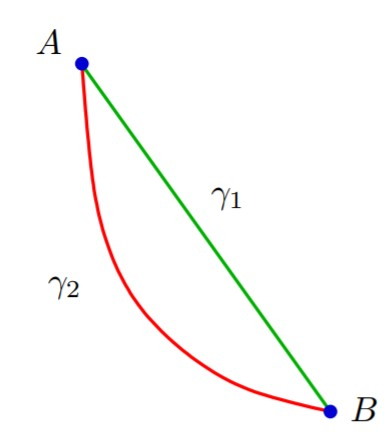
\includegraphics[width=2.5cm]{brachi}
		\caption{example of two trajectories $\gamma_1,\gamma_2$ that an object can follow for moving from point $A$ to $B$.}
	\end{SCfigure}
	
	Mathematically the problem is determining the curve $\mathcal C: [a,b] \rightarrow \mathds R$ such that $\mathcal C(a) = y_a$ and $\mathcal C(b) = y_b$ that minimize the function $T(\mathcal C)$ representing the time to travel and so
	\[ \textrm{minimize } T(\mathcal C) \qquad \textrm{for all possible curves } \mathcal C \]
	
	We can see that a \textbf{function} takes a number as input and returns a number, like $f(x) = x e^x$. A \de{functional} is instead something that takes as input a function and returns a number and an example is
	\[ \mathcal F (x) = \int_a^b x(t)\, dt  \]
	where $x$ is a function. Considering for example $x(t) = t^2$ the previous functional  becomes
	\[ \fun F(x) = \int_a^b t^2\, dt = \left. \frac{t^3}{3}\right|_a^b= \frac{b^3-a^3}{3}\]
	
	Another example of functional can be $\fun G(z) = z'(0) \int_0^1 z^2(t)\, dt$ and this expression can be evaluated for every generic function $z(t)$.	\vspace{3mm}
	
	The question of this problem is how to define a \textit{minimum} for a functional; in order to do so we have to firstly understand how to minimize a simple function and in particular given a function $f: A\subseteq \R \rightarrow \R$ has a minimum in the point $x^*$ if
	\[  f(x^*) \leq f(x) \qquad \forall x \in A \]
	Similarly given a function $\fun F(x)$ a \textit{point} $x^*$ (that in reality is a function) is a minimum if 
	\[ \fun F(x^*) \leq \fun F(x) \qquad \forall x \in ? \]
	In this case we have to specify the \textit{class} (functional space) of functions we are considering, as example $x$ can be a function that's continuous in the domain $[a,b]$ and so we can define
	\[ x\in C([a,b]) = \big\{ g:[a,b]\rightarrow R \ | \ g \textrm{ is continuous} \big\} \]
	In general changing the \textit{domain} of the functional $\fun F$ may change the problem.
	\begin{example}{: domain change}
		Considering the function $f(x) = x^2+2$, it's roots can be computed if we allow complex solutions $z\in \mathds C$ (and in fact $z = \pm i \sqrt 2$), while if the domain of the solution is the real set $z\in \R$ no solutions exists. \vspace{3mm}
		
		Considering now the functional $\fun F$ defined as
		\[ \fun F(x) = \int_{-1}^1 \big(x(t) - |t|\big)^2\, dt \]
		The $|t|$ introduce a cuspid in $t=0$ that cannot be derived. If we minimize the functional in the continuous interval $x\in C([-1,1])$, the solution is the function $x^*(t) = |t|$, in fact
		\[ \fun F(x^*) = \int_{-1}^1 \big(|t|-|t|\big)^2 \, dt = \int_{-1}^1 0\, dt = 0 \]
		Choosing any other continuous function will result in a functional with a positive value.
		
		Considering now to minimize the function in the domain of functions with continuous derivatives, and so $x\in C^1([-1,1])$. In this case $|t|\notin C^1([-1,1])$ (due to the cuspid). An approximation of the function $|t|$ that is continuous with also continuous first derivative is the function
		\[ x_\varepsilon(t) = \begin{cases}
			t \qquad & t \geq \varepsilon \\
			\frac 1 2 \left(\frac{t^2}\varepsilon + \varepsilon\right) \qquad & -\varepsilon < t< \varepsilon \\
			-t & t \leq- \varepsilon
		\end{cases} \]
		By pushing the limit $\varepsilon\rightarrow 0$ we can have the function that minimize the functional $\fun F$ in the domain $C^1([-1,1])$. In fact we can see that the functional of $x_\varepsilon$ becomes
		\[ \fun F(x_\varepsilon) = \int_{-\varepsilon}^\varepsilon \left( \frac{t^2}{2\varepsilon} + \frac \varepsilon 2 - |t| \right)^2\, dt = \frac{\varepsilon^3}{10} \]
		
	\end{example}

\section{Analogies with linear algebra}
	To solve the problem of minimizing a functional we can see some relations with the linear algebra. The domain of the functional can be in fact see as a \de{functional space} $\mathds V$ analogous to the vectorial one which the vectors are represented by the functions and the scalars are represented by real values. With this definition example of functional spaces might be
	\[ \mathds V_1 = \big\{ f : [0,1] \rightarrow \R \textrm{ continuous}\big\} \]
	\[ \mathds V_2 = \big\{ f: [a,b]\rightarrow \R \textrm{ such that } f\in C^k([a,b]) \big\} \qquad \textrm{with } a,b \in \R, \ k\in \mathds N \]
	Given in fact two function $f,g \in \mathds V$ that are member of the same functional space, we can see that each linear combination of the functions determine a function that's still in the vectorial space:
	\[ \alpha f(x) + \beta f(x) \in \mathds V \qquad \forall \alpha,\beta \in \R, \ f(x),g(x) \in \mathds V \]
	As example let's consider the two continuous function $f(x) = x^2$ and $g(x) = \sin x$, then we can clearly see that the function $2f(x) + \frac 13 g(x) = 2x^2 +\frac 13\sin x$ is still continuous. This in general means that the functional space is \textit{closed} respect to the operations of function summation and multiplication by a scalar.
	
	\paragraph{Scalar product} In linear algebra given two vector $\vett v_1, \vett v_2$ it exists the bilinear operator scalar product $\langle \vett v_1,\vett v_2 \rangle = \vett v_1 \cdot \vett v_2$  that satisfy the following rules:
	\[ \langle \alpha \vett v + \beta \vett w, \vett z\rangle = \langle \vett z , \alpha \vett v + \beta \vett w\rangle = \alpha \langle \vett v,\vett z\rangle + \beta \langle \vett w,\vett z\rangle \qquad \forall \alpha,\beta \in \R, \ \vett v,\vett w,\vett z \in \mathds V \]	
	\[ \langle \vett v,\vett v\rangle \geq 0 \qquad \textrm{ and } \qquad \langle \vett v,\vett v \rangle = 0 \quad \Leftrightarrow \quad \vett v = \vett 0 \]
	
	Also in the functional space $\mathds V$ can exists definitions of product scalar such the one here presented:
	\begin{equation} \label{eq:func:pscalexample}
		\langle f,g\rangle = \int_0^1 f(x)g(x)\, dx
	\end{equation}
	\begin{note}
		This is not the lonely function that can serve as product scalar of function and in this case the relation holds for the functional space $\mathds V = \{ f:[0,1] \rightarrow \R \textrm{ integrable} \}$.
	\end{note}
	In this case we can prove that this definitions meets the requirements stated for the scalar product considering the linear properties of the integrals as follows:
	\begin{align*}
		\langle \alpha f(x) + \beta g(x),h(x) \rangle & = \int_0^1 \Big(\alpha f(x) + \beta g(x)\Big)h(x) \, dx \\ 
		& = \alpha \int_0^1 f(x)h(g) \, dx + \beta \int_0^2 g(x)h(x) \, dx \\
		& = \alpha \langle f(x),h(x) \rangle + \beta \langle g(x),h(x) \rangle
	\end{align*}
	and also
	\[ \langle f(x),f(x) \rangle = \int_0^1 f(x) f(x) \, dx = \int_0^1 f^2(x)  \geq 0  \]
	and in particular we can see that the scalar product $\langle f(x),f(x)\rangle$ will give as result 0 if and only if the function $f$ is identically null, so such that $f(x) = 0$ for all $x$ in it's domain (in this case $[0,1]$).
	
	\paragraph{Norm} In linear algebra it's also defined the norm of a vector as
	\[ \|\vett v\| := \sqrt{\vett v \cdot \vett v} \]
	and this expression is used to compute, from a vector, a single positive value  (and in particular $\|\vett v\| = 0$ if and only if $\vett v = \vett 0$). This definition also holds for the functional space and considering the scalar product defined (as example) in equation \ref{eq:func:pscalexample} we can see that one definition of norm for function can be the one
	\[ \|f(x)\| = \sqrt{\langle f(x),f(x)\rangle} = \sqrt{\int_0^1f^2(x) \, dx} \]
	In this case we can clearly see that the norm $\|f(x)\| \geq 0$ is always positive defined (and is zero only in the case on which the function $f$ is identically null).
	
	
	\begin{example}{: space of function}
		A space of functions can ve the one $f:[a,b]\rightarrow \R$ such that $f$ is continuous, or for example $f:[a,b]\rightarrow \R$ where $f\in C^k([a,b])$ (for $k\in \mathds N$). The same can be said for piecewise continuous functions.
		
		Less trivially is a space of function the set of $f:[a,b]\rightarrow \R$ that are module integrable, and so all the function $f$ such that
		\[\int_a^b |f(x)|\, dx < \infty\]
		
	\end{example}

	In general we define as $L^p([a,b])$ the space of $p$-integrable functions, so such that
	\[ f\in L^p([a,b])  \qquad \Leftrightarrow \qquad \int_a^b |f(x)|^p\, dx < \infty\]
	
	
\section{Directional derivative} 
	Given a bidimensional function $f:\R^2\rightarrow \R$ in the variable $x,y$ a point $(x\s,y\s)$ is a global minimum if it satisfy the following relation:
	\[ f(x\s,y\s) \leq f(x,y) \qquad \qquad \forall (x,y)\in \R^2 \]
	
	Given so a direction defined by the vector $\vett d = (dx,dy)$ it's possible to reconduct the multi valued function $f$ into a one dimensional function $g$ as
	\[ g(t) = f\big( x\s + t\, dx,y\s + t\, dy \big)  \]
	With this definition we can see that $g(0)$ corresponds to $f(x\s,y\s)$ and so for any other value of $t$ it happens that $g(t) \geq f(x\s,y\s)$ (based on the assumption that $(x\s,y\s)$ is the global minimum of the function $f$). This also means that the relation $g(t)-g(0) \geq 0$ for all value of $t \geq 0$: dividing this relation by the parameter $t$ and pushing the limit for the variable approaching zero will give the analytical result of the derivative of $g$ evaluated at zero
	\begin{equation} \label{eq:func:directional}
		g'(0) := \lim_{t\rightarrow 0} \frac{g(t) - g(0)}{t} \geq 0 
	\end{equation}
	
	If the function $f$ also presents a Taylor series expansion of the first order respect to the point $(x\s,y\s)$ of global minimum it can be written as
	\[ f\big( x\s + t\, dx, y\s +t \, dy\big) = f\big(x\s,y\s\big) +\nabla f\big(x\s,y\s\big) \vector{t \,dx \\ t\, dy} + \mathcal O(t^2) \]
	Rearranging this expression on the by shifting to the left the term $f(x\s,y\s)$ and dividing by $t$ it's possible to observe the relation to the directional derivative (equation \ref{eq:func:directional}) as
	\begin{align*}
		\frac{g(t)-g(0)}{t} & = \frac{f( x\s + t\, dx, y\s +t \, dy)  - f(x\s,y\s)}{t} \\
		& = \nabla f\big(x\s,y\s) \vector{dx \\ dy} + \cancel{\mathcal O(t)}
	\end{align*}
	As shown previously it must be that the directional derivative $g'(0) = \nabla f(x\s,y\s) \vett d \geq 0$ must be greater or equal to zero. Considering however as direction on which compute the derivative the opposite of the one determined by the gradient, so $\vett d = - \nabla f(x\s ,y\s)^t$, we can see that the product becomes
	\[ \nabla f(x\s,y\s) \big(-\nabla f(x\s,y\s)^t\big) = - \| f(x\s,y\s)\|^2 \]
	We can now see that the lonely way to have $-\|f(x\s,y\s)\geq 0$ is having a function $f$ such that it's gradient  is identically null, and so $\nabla f(x\s,y\s) = \vett 0$.
	
\subsection{Stationary points for a functional}
	Until now we defined a functional $\mathcal F: \mathds V \rightarrow \R$ a type of function that relate function of the functional space $\mathds V$ with real values in $\R$. Let $x\s(t)$ a function that \textit{minimize} the functional $\mathcal F(x)$ and consider $y(t)$ another \textit{point} (function) in the functional domain: this means that
	\[ \F(x\s) \leq \F(y) \]
	
	In this functional space we can determine a line that connects the points determined by $x\s$ and $y$ creating a \textit{linear interpolation}, generating a new function $z(t,\tau)$ as a linear combination of the original points:
	\[ z(t,\tau) :=  x\s(t) + \tau \underbrace{\big( y(t) - x\s(t) \big)}_{=d(t) \textrm{: direction}} \]
	We can see that for $\tau = 0$ the function $z$ reduces to the minimum point $x\s$, while for $\tau = 1$ it matches the other point $y$; the difference $y(t)-x\s(t) = d(t)$ indeed represents the direction on which the two functions combines.
	
	With that said it's possible to compute a \textit{slice} $g(\tau)$ of the original functional $\F$ along the direction determined by the function $z(\cdot,\tau)$ and so
	\begin{equation}
		g(\tau) := \F\big( z(\cdot,\tau) \big) = \F\big(x\s + \tau d\big)
	\end{equation}
	We can see that the function $g$ maps a real value $\tau\in\R$ into another real value, and in particular considering the initial assumption of $x\s$ being a minimal point of $\F$ it means that
	\[ g(0) = \F(x\s) \leq g(\tau) = \F(x\s + \tau d) \]
	Considering this relations and assuming that's possible to compute the derivative of $g$, evaluating it for the point $\tau = 0$ will get the results:
	\begin{align*}
		g'(0) & = \lim_{\tau\rightarrow 0^+} \frac{g(\tau)-g(0)}{\tau} \geq 0 \\
		& = \lim_{\tau\rightarrow 0^-} \frac{g(\tau)-g(0)}{\tau} \leq 0 
	\end{align*}
	and so this means, in order to have a continuous derivative for $\tau = 0$ that the \textbf{derivative must be null}:
	\[ \Rightarrow \qquad g'(0) = 0 \]
	
	The conclusion of this process is that a function $x\s$ to be a minimum point must present a directional derivative that's equal to zero for each feasible direction $d$ that we consider.
	
	
	\begin{example}{: directional derivative of a functional}
		Given the functional
		\[ \fun F(x) = \int_0^1 \Big(x^2(t) + 1\Big) \, dt  \ + x(1) \]
		it's  possible to compute the directional derivative in $x(t)$ with direction $d(t)$ by firstly determining the function $g:\R\rightarrow \R$ that's the evaluation of the functional for the function $z(t,\alpha) = x(t) + \alpha \, d(t)$:
		\begin{align*}
			g(\alpha) & = \F \big(z(t,\alpha)\big) = \F\big(x(t) + \alpha\, d(t)\big) \\
			& = \int_0^1 \Big( \big(x(t) + \alpha\, d(t)\big)^2 + 1 \Big)\, dt  + x(1) + \alpha\, d(1)
		\end{align*}
		Deriving this expression respect to the parameter $\alpha$ will give the function
		\[ g'(\alpha ) = \frac{dg(\alpha)}{d\alpha} = \frac d{d\alpha } \int_0^1 \Big( \big(x(t) + \alpha\, d(t)\big)^2 + 1 \Big)\, dt  +  \frac d{d\alpha} \Big(x(1) + \alpha\, d(1)\Big) \]
		
		Assuming that $\frac d{d\alpha}\int = \int \frac d{d\alpha}$ (operation that cannot always be performed) this expression reduces to a form that's easier to evaluate:
		\begin{align*}
			g'(\alpha) &= \int_0^1 \frac d{d\alpha} \Big(x(t) + \alpha\, d(t)\Big)^2\, dt + \frac d{d\alpha} \Big(x(1) + \alpha \, d(1)\Big) \\
			& = \int_0^1 2\big(x(t) + \alpha\, d(t)\big) d(t)\, dt + d(1) \\
			g'(0)& = \int_0^1 2x(t)d(t)\, dt + d(1)
		\end{align*}
		and so the directional derivative of the original functional $\F$ respect to the direction $d(t)$ is determined by $g(0)$.
	\end{example}
	
\section{Fundamental lemma of the calculus of variations}
	{\itshape Given a function $f:[a,b]\rightarrow \R$ (piecewise continuous) such that for all $g:[a,b] \rightarrow \R$ continuous (and more in particular $g \in C^\infty([a,b])$ to have a more general definition ) with $g(a) = g(b) = 0$ and $g^{(k)}(a) = g^{(k)}(b) = 0 \ \forall k$, if the integral 
	\begin{equation} \label{eq:func:lemma}
		\int_a^b f(x)\,g(x) \, dx = 0
	\end{equation}
	then $f(x)= 0 $ is identically null. }

	\paragraph{Lemma: sign permanence} In order to later proof the fundamental lemma yet described, we have to remark the \textit{sign permanence} that states: {\itshape given a function $f:[a,b]\rightarrow \R$ continuous such that $f(c) >0$, then there exists a $\delta >0$ such that }
	\[ f(x) \geq \frac{f(c)}{2} \qquad \forall x \in [c-\delta,c+\delta] \]
	
	The proof of this lemma can be done defining the parameter $\epsilon = f(c) / 2$; based on the assumption that $f(x)$ is continuous, then
	\[ \exists \delta >0 \qquad \textrm{such that} \qquad |f(x) - f(c)| \leq \varepsilon = \frac{f(c)}{2} \qquad \forall |c-x|\leq \delta \]
	Expanding the module operation the inequality becomes:
	\[ -\frac{f(c)}{2} = - \epsilon \leq f(x)-f(c) \leq \epsilon = \frac{f(c)}{2} \]
	\[ \Rightarrow \qquad \underbrace{-\frac{f(c)}{2} + f(c) \leq f(x)}_{\frac{f(c)}{2} \leq f(x)} \leq f(c) + \frac{f(c)}{2} \]
	and so we prove the lemma of sign permanence.
	
	\paragraph{Proof of the fundamental lemma} The proof of the fundamental lemma of the calculus of variation can be done by contradiction. Let consider the integral $\int_a^b f(x) g(x)\, dx = 0$ for all functions $g(x)$ and such that, given the function $f$, exists a point $c$ such that $f(c) > 0$ (in general the proof can be done for $f(c)\neq 0$). from the sign permanence lemma we can state that exists an interval $[c-\delta,c+\delta]$ such that $f(x) \geq \frac{f(c)}{2 } \geq 0$. Determining the function $g$ as
	\[ g(x) = \begin{cases}
		\dfrac{x-(c-\delta)}{\delta} \qquad & x\in [c-\delta, c] \\
		\dfrac{c-x+\delta}{\delta} & x\in[c,c+\delta] \\
		0 & \textrm{otherwise}
	\end{cases} \]
	Note that this function is continuous but $g\notin C^\infty$ (later will be described a function that presents this feature). With this definition the integral $\int_a^b fg\, dx$ so becomes
	\begin{align*}
		\int_{c-\delta}^{c+\delta} f(x)g(x)\, dx & \geq \frac{f(c)}{2} \int_{c-\delta}^{c+\delta} g(x)\, dx \\
		& \geq \frac{f(c)}{2}\frac \delta 2 > 0
	\end{align*}
	We can clearly see that the integral $\int_a^b fg\, dx$ has a positive real value grater than zero that's (considering that $f$ has at least on point $c$ such that $f(c) >0$) in contraposition with the initial request that the integral should have been zero evaluated. \vspace{3mm}
	
	To create a direction function $g$ that's in the set $C^\infty$ we can use the function $h$(for whose those condition is demonstrated) as in figure \ref{fig:func:ht} defined as:
	\begin{equation} \label{eq:func:ht}
		h(t) = \begin{cases}
			e^{-1/t} \qquad & t > 0 \\ 
			0 & t\leq 0
		\end{cases}
	\end{equation}
	\begin{SCfigure}[2][bt]
		\centering 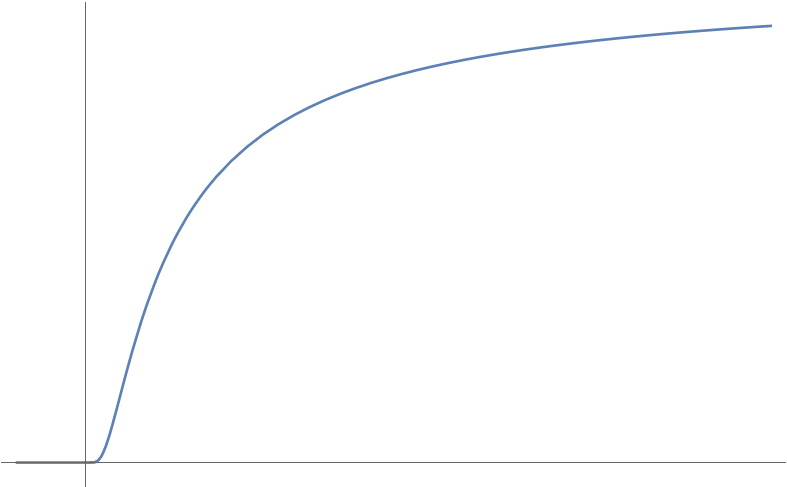
\includegraphics[width=4cm]{cinf-a}
		\caption{representation of $h(t)$ defined in equation \ref{eq:func:ht}}.
		\label{fig:func:ht}
	\end{SCfigure}

	A way to create a function that presents a \textit{bell shape} in the range $[0,1]$ is by computing $g(t) := h(t) h(1-t)$ how's graph in the range $[0,1]$ is similar to the one shown in figure \ref{fig:func:hbell}.
	
	\begin{SCfigure}[2][bht]
		\centering 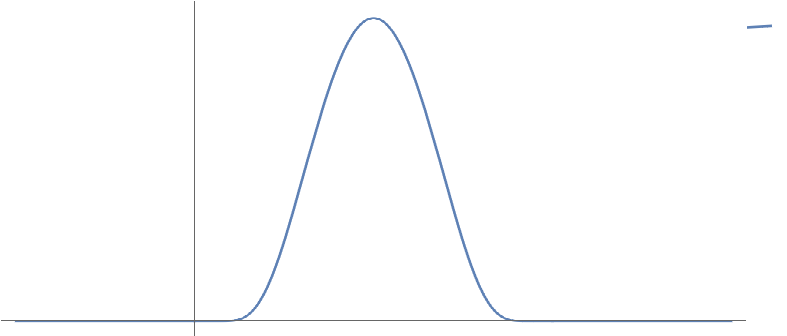
\includegraphics[width=4cm]{cinf-b}
		\caption{representation of the function $g(t):=h(t)h(1-t)$, where $h(t)$ is defined in equation \ref{eq:func:ht}}.
		\label{fig:func:hbell}
	\end{SCfigure}
	
	In particular to demonstrate the fundamental lemma of the calculus of variations we need to rescale the function $g$ in order to have a bell centered in the point $c$ with a \textit{bell width} $\delta$ and so we consider
	\[ g(t) = K \, h\left(\frac{t-c+\delta}{2 \delta}\right) h\left( \frac{\delta + c - t}{2 \delta} \right) \] 
	where the constant $K\in\R$ is such that $g(c)=1$ and $\int_a^bg(x)\, dx$. In this case we can see that $g\in C^\infty$, $g(x) \geq 0 $ for all value $x$ and specifically $g(x) = 0 \, \forall x\notin[c-\delta,c+\delta]$.\\
	The lemma can now be proven by contradiction; as in the previous case if we consider a function $f$ that's not identically null (and in this case we assume that there is at least one point $c$ on which $f$ is positive), then we can state that (for the sign permanence theorem)
	\[ f(x) \geq \frac{f(c)}{2} \qquad \forall x \in [c-\delta,c+\delta] \] 
	We can now see that the original integral $\int_a^b fg\, dx$ is not equal to zero, in fact
	\[ \int_a^b f(x)g(x)\, dx \geq \frac{f(c)}{2}\int_a^bg(x)\, dx > 0 \]
	because $g(x)$ is always greater or equal to zero, determining a non zero value as result as in the previous case.
	
\section{Euler Lagrange equation}
	\paragraph{Pendulum example} The \de{Euler Lagrange equation} is the generalization of the minimum action principle that's used in physics. Considering as a practical example the motion of a pendulum of a mass $m$ that's free to oscillate in respect to a pivot point using a rope of length $l$, the kinetic energy $T$ and the potential term $V$ of the system can be expressed as
	\[ T = \frac 1 2 m v^2 \qquad \qquad \qquad V = mgy \]
	Considering $\theta$ as the angle that the rope determines with the vertical axis, then the we can rewrite the energies as functions of the angular position $\theta$ and velocity $\dot \theta$ as
	\[ T(\theta,\dot \theta) = \frac 1 2 m l^2 \dot\theta^2 \qquad \qquad \qquad V(\theta) = - m gl\sin\theta \]
	
	To solve the dynamic equation $\theta(t)$ of the mechanism we can compute the lagrangian $\mathcal L$ of the system defined as
	\[ \mathcal L(\theta,\dot\theta) = T(\theta,\dot\theta)-V(\theta) = \frac m 2 l^2\dot\theta^2 + lmg\cos\theta \]
	As law that's analyzed in mechanics physics we can state that the solution of the dynamics of the system is the one the function that minimize the \textbf{action} $\mathcal A$ of the system defined as
	\begin{equation} \label{eq:func:action}
		A(\theta) = \int_{t_0}^{t_1} \mathcal L(\theta,\dot\theta)\, dt
	\end{equation}
	where the values $\theta(t_0)= \theta_0$ and $\theta(t_1)=\theta_1$ are known parameters.
	
	In practice to determine the required solution we can use analytical tool to find the trajectory that can then be demonstrated to be the minimum of the action $\mathcal A$ (that's indeed a functional).
	
	However we can also try to analytically determine the function $\theta^*(t)$ that minimize the functional $\fun A(\cdot)$ by computing the directional derivatives. \vspace{3mm}
	
	Let now consider the function $\theta\s(t)$ and a direction $\delta_\theta$ that satisfy $\delta_\theta(t_0)=\delta_\theta(t_1) = 0$, we can then use the fundamental lemma of the calculus of variation to determine the minimal function (considering that the expression \ref{eq:func:action} of the action is comparable to equation \ref{eq:func:lemma} of the lemma).\\
	To determine the minimum point we have in fact to determine the function whose derivative is zero for each direction of approach to the point, and so in this example we need to compute
	\begin{align*}
		\frac{d}{d\alpha} \mathcal A\big(\theta\s + \alpha\, \delta_\theta\big) & = \frac{d}{d\alpha}\int_{t_0}^{t_1} \mathcal L \big( \theta \s + \alpha\, \delta_\theta, \dot\theta\s + \alpha\, \dot \delta_\theta \big) \\
		& = \int_{t_0}^{t_1} \left[\pd{}{\theta} \mathcal L( \dots ) \frac{d}{d\alpha}\big(\theta\s + \alpha \,\delta_\theta\big) +\pd{}{\dot\theta} \mathcal L (\dots) \frac{d}{d\alpha}\big(\dot \theta\s + \alpha \,\dot \delta_\theta\big) \right]\, dt \\
		& = \int_{t_1}^{t_2} \left[ \big(-lmg\sin(\theta\s + \alpha\, \delta_\theta)\big)\delta_\theta + ml^2\big(
		\dot\theta\s + \alpha \, \dot\delta_\theta \big)\, \dot\delta_\theta \right] \, dt
	\end{align*}
	Note that from in the first step we made the implicit assumption that $ \frac d{d\cdot} \int = \int\frac{d}{d\cdot}$ while however this is not always possible. Evaluating the previous expression for $\alpha = 0$ we can state that
	\[ 	\frac{d}{d\alpha} \mathcal A\big(\theta\s + \alpha\, \delta_\theta\big) \Big|_{\alpha = 0} = \int_{t_0}^{t_1} \big(-lmg \sin\theta\s\delta_\theta + ml^2\dot\theta\s \dot\delta_\theta \big) \, dt = 0 \qquad \forall \delta_\theta \]
	Performing an integration by part allows to remove the term $\dot\delta_\theta$ that's hard to determine, and in fact
	\[ \frac{d}{dt}\big( ml^2\dot\theta\s \, \delta_\theta\big) = \frac{d}{dt}\big(ml^2\dot\theta\s\big)\,\delta_\theta + ml^2\dot\theta\s \dot\delta_\theta\]
	\begin{align*}
		\Rightarrow \quad \left. \frac{d\mathcal A}{d\alpha}\right|_{\alpha = 0} & = \int_{t_0}^{t_1}  \left[ - lmg\sin\theta\s - \frac d{dt}\big(ml^2\theta\s\big)^2 \right]\delta_\theta\, dt + \cancel{\big[ ml^2 \dot\theta\s \delta_\theta \big]\Big|_{t_0}^{t_1} } \\
		& = \int_{t_0}^{t_1} \underbrace{\left[ -lmg \sin\theta\s - \frac d{dt}\big(ml^2 \dot\theta\s\big) \right]}_{f(t)} \delta_\theta\, dt = 0
	\end{align*}
	We can now see in this formulation that the marked expression represent the function $f$ of the fundamental lemma considering that the relation must be true for all approaching direction $\delta_\theta$, and so it must be
	\[ -lmg \sin\theta\s - \frac d{dt}\big(ml^2 \dot\theta\s\big) = 0 \]
	The problem now to complete the analyses of the pendulum motion is determining the function $\theta\s(t)$ that satisfy this expression and also match the boundary conditions $\theta(t_0) = \theta_0$ and $\theta(t_1)=\theta_1$.
	
\subsection{General formulation} \label{sec:func:eullag}
	Given a functional
	\begin{equation}
		\mathcal A(x) = \int_a^b \mathcal L\big(x(t),x'(t),t\big)\, dt
	\end{equation}
	the problem is to minimize the functional $\mathcal A$ for a function $x \in \mathds V$ such that $x(a) = x_a$ and $x(b) = x_b$ where the function space $\mathds V$ is defined as
	\[ \mathds V = \big\{ x \ | \ x\in C^2([a,b]) \textrm{ with } x(a) = x_a,x(b) = x_b \big\} \]
	Let $\mathds D$ the function space of all the feasible directions of derivatives defined as
	\[ \mathds D = \big\{ \delta_x \ | \ \delta_x \in C^{\infty}([a,b]) \textrm{ with } \delta_x(a) = \delta_x(b) = 0 \big\} \]
	the function $x(t)$ that minimize the functional is the one whose derivative respect to $\alpha$ is always zero (for $\alpha = 0$) for any feasible direction for the derivative, and so 
	\[ x(t) \quad\textrm{such that} \quad \frac{d}{d\alpha} \mathcal{A}(x+\alpha\, \delta_x) \Big|_{\alpha = 0} = 0 \qquad \forall \delta_x \in \mathds D \]	
	
	Assuming the possibility to correctly apply the rule $\frac{d}{d\cdot} \int = \int \frac{d}{d\cdot}$ we can express the derivative of the functional $\mathcal A$ evaluated in $x+ \alpha\, \delta_x$ as
	\begin{align*}
		\frac{d\mathcal A}{d\alpha} & = \frac{d}{d\alpha} \int_a^b \mathcal L\big( x + \alpha\, \delta_x ,x' + \alpha\, \delta_x', t\big)\, dt \\
		& = \int_a^b \left(\pd{\mathcal L}x \delta_x + \pd{\mathcal L}{x'} \delta_x'\right)\, dt \\
		\left. \frac{d\mathcal A}{d\alpha} \right|_{\alpha = 0} & = \int_a^b \left( \pd{\mathcal L(x,x',t)}x \delta_x + \pd{\mathcal L(x,x',t)}{x'} \delta_x' \right)\, dt 
	\end{align*}
	By performing the integration by part it's possible do reconvert the term associated do $\delta_x'$ into pieces depending on $\delta_x$ one of which, when evaluated, becomes zero due to the fact that $\delta_x(a) = \delta_x(b) = 0$:
	\begin{align*}
		\left. \frac{d\mathcal A}{d\alpha} \right|_{\alpha = 0} & = \int_a^b \left[ \pd{\mathcal L(x,x',t)}{x} - \frac{d}{dt} \left( \pd{\mathcal L(x,x',t)}{x'} \right) \right] \delta_x\, dt + \int_a^b\frac{d}{dt}\left( \pd{\mathcal L(x,x',t)}{x'}\delta_x \right) \, dt \\
		& = \int_a^b \left[ \pd{\mathcal L(x,x',t)}{x} - \frac{d}{dt} \left( \pd{\mathcal L(x,x',t)}{x'} \right) \right] \delta_x\, dt + \cancel{\left. \left[ \pd{\mathcal L(x,x',t)}{x'}\delta_x \right] \right|_{\delta_x = a}^b} \\
	\end{align*}
	We can now see that the condition to have a minimum for the functional $\mathcal A$, by using the fundamental lemma of calculus of variation, is requiring that the function $f$ defined as follows is identically null:
	\begin{equation} \label{eq:func:var1}
		\left. \frac{d\mathcal A(x+\alpha\, \delta_x)}{d\alpha} \right|_{\alpha = 0} = \int_a^b \underbrace{\left(\pd{\mathcal L}{x} - \frac d{dt}\pd{\mathcal L}{x'}\right)}_{=f} \delta_x \, dt = 0
	\end{equation}
	
	This in general means that the function that minimise the functional $\mathcal A$ must solve the following second order ordinary differential equation:
	\[ \begin{cases}
		\dfrac d{dt} \dfrac{\partial\mathcal L}{\partial x'} - \dfrac {\partial \mathcal L}{\partial x} = 0 \\ x(a) = x_a \, ,\ x(b) = x_b
	\end{cases} \]
	
	\paragraph{Definitions} Given a functional $\F$ we define the directional derivative
	\[ \frac{d}{d\alpha} \F(x+\alpha\, \delta_x) \]
	of the functional evaluated on the function $x$ with direction $\delta_x$ as \de{Gateaux derivative} and we simplify the operation of evaluating the derivative for $\alpha= 0$ with the letter $\delta$ as
	\begin{equation}
		\delta \F(x) := \frac{d}{d\alpha} \F\big(x+\alpha\, \delta_x\big) \Big|_{\alpha = 0}
	\end{equation}
	This definition is also referred as the \de{first variation} of the functional $\F(x)$. \vspace{3mm}
	
	Considering now the functional
	\[ \F(x) = \int_a^b \fun G(x,x',t)\, dt + x(a)x(b) \]
	using the \textit{standard} approach until now used, to search for the minimum solution we have to compute the directional derivative evaluating it at the point $\alpha = 0$:
	\begin{align*}
		&= \frac d{d\alpha} \F \big(x+\alpha\, \delta_x\big) \Big|_{\alpha=0} \\
		&= \frac{d}{d\alpha}\left( \int_a^b \mathcal G\big(x+\alpha\, \delta_x, x' + \alpha\, \delta_x',t\big)\, dt  + \Big(x(a) + \alpha \delta_x(a)\Big)\Big(x(b) + \alpha\, \delta_x(b)\Big) \right) \\
		&=  \int_a^b \left( \pd{\mathcal G(\dots)} x \, \delta_x + \pd{\mathcal G(\dots)} {x'} \delta_x' \right) \, dt  + \delta_x(a) \Big(x(b) + \alpha\, \delta_x(b)\Big) + \Big( x(a) + \alpha\,\delta_x(a) \Big)\delta_x(b) \\
		&=  \int_a^b \left( \pd{\mathcal G(\dots)} x \, \delta_x + \pd{\mathcal G(\dots)} {x'} \delta_x' \right) \, dt  + \delta_x(a)x(b) + x(a)\delta_x(b)
	\end{align*}
	Using instead the Gateaux notation for the derivative the same problem can be simplified in the notation as
	\begin{align*}
		&= \delta \F(x) \\
		&= \delta \left(\int_a^b \fun G(x,x',t)\, dt + x(a)x(b)\right) \\
		&= \int_a^b \delta \mathcal G(x,x',t)\, dt + \delta_x(a) x(b) + x(a)\delta_x(b) \\
		&= \int_a^b \left( \pd{\mathcal G(x,x',t)}{x}\delta_x + \pd{\mathcal G(x,x',t)}{x'} \delta_x' \right)\, dt + \delta_x(a) x(b) + x(a)\delta_x(b)
	\end{align*}

\subsection*{Extended definition}
	Considering now the functional $\mathcal B$ defined as
	\begin{equation} \label{eq:func:lag2}
		\mathcal B(x) = \int_a^b \mathcal L(x(t),x'(t),x''(t),t)\, dt
	\end{equation}
	the problem to solve now is the minimization of $\mathcal B(x)$ for all the function $x\in \mathds V$ where the functional space is defined as
	\[ \mathds V = \left\{ x \textrm{ such that } \begin{aligned}
		& x\in C^4([a,b]) \\ & x(a) = x_a, x'(a) = x_a', x(b) = x_b, x'(b) = x_b'
	\end{aligned} \right\} \]
	and directional derivatives $\delta_x \in \mathds D$ in the functional domain
	\[ \mathds D = \left\{ \delta_x \textrm{ such that } \begin{aligned}
		& x\in C^\infty([a,b]) \\ & x(a) = x'(a) = x(b) = x'(b) = 0
	\end{aligned} \right\} \]
	
	When trying to calculate the directional derivative of the functional $\mathcal B$ (skipping all the unnecessary computation that's similar to the cases yet studies) we end up to the following results:
	\begin{align*}
		& = \left.\frac{d}{d\alpha}\right|_{\alpha = 0} \mathcal B(x+\alpha, \delta_x) \\
		& = \left. \frac{d}{d\alpha}\right|_{\alpha = 0} \int_a^b \mathcal L\big( x + \alpha\, \delta_x, x' + \alpha\, \delta_x', x''+\alpha\, \delta_x'',t\big) \, dt \\
		& = \int_a^b \left( \pd{\mathcal L(x,x',x'',t)}{x}\delta_x + \pd{\mathcal L(x,x',x'',t)}{x'}\delta_x' + \pd{\mathcal L(x,x',x'',t)}{x''}\delta_x'' \right) \, dt
	\end{align*}
	To \textit{cancel out} the terms involving the terms $\delta_x',\delta_x''$ it's necessary to use integration by parts considering the following derivatives:
	\[ \frac d{dt} \left(\pd{\mathcal L}{x'}\, \delta_x \right) = \frac d{dt} \pd{\mathcal L}{x'} \delta_x + \pd{\mathcal L}{x'} \delta_x' \qquad \qquad \frac d{dt} \left(\pd{\mathcal L}{x''}\, \delta_x' \right) = \frac d{dt} \pd{\mathcal L}{x''} \delta_x' + \pd{\mathcal L}{x''}\delta_x''  \]
	and so with that said the derivative becomes
	\begin{align*}
		\delta \mathcal B& = \int_a^b \left( \pd{\mathcal L}{x}\delta_x + \cancel{\frac d{dt} \left(\pd{\mathcal L}{x'} \delta_x \right)} -  \frac{d}{dt} \pd{\mathcal L}{x'} \delta_x + \cancel{\frac d{dt}\left( \pd{\mathcal L}{x''} \delta_x' \right) } - \frac{d}{dt} \pd{\mathcal L}{x''} \delta_x' \right)\, dt \\
		& = \int_a^b \left[\left( \pd{\mathcal L}{x}  -  \frac{d}{dt} \pd{\mathcal L}{x'} \right)\delta_x - \frac{d}{dt} \pd{\mathcal L}{x''} \delta_x' \right]\, dt
	\end{align*}
	In the first line the terms are cancelled because if evaluated singularly we can see that they become in the form
	\[ \int_a^b \frac d{dt} \left(\pd{\mathcal L}{x'} \delta_x\right) \, dt = \left. \left[ \pd{\mathcal L}{x'} \delta_x \right]\right|_a^b \xrightarrow{\delta_x(a) = \delta_x(b) = 0} 0  \]

	To finish the analysis of the derivation we have to consider one last integration by part for the element
	\[ \frac{d}{dt} \left( \frac{d}{dt} \pd{\mathcal L}{x''} \delta_x \right) = \frac{d^2}{dt^2} \pd{\mathcal L}{x''} \delta_x + \frac{d}{dt} \pd{\mathcal L}{x''} \delta_x' \]
	\begin{equation} \label{eq:func:var2}
		\Rightarrow \qquad \delta\mathcal B(x) = \int_a^b \underbrace{\left( \pd{\mathcal L}{x} - \frac d {dt} \pd{\mathcal L}{x'} + \frac{d^2}{dt^2} \pd{\mathcal L}{x''} \right)}_{=f} \delta_x\, dt
	\end{equation}
	Using so the fundamental lemma of calculus of variation in order to determine the function $x$ that minimize the functional $\mathcal B$ we need to solve the system of differential equation
	\[   \pd{\mathcal L}{x} - \frac d {dt} \pd{\mathcal L}{x'} + \frac{d^2}{dt^2} \pd{\mathcal L}{x''} = 0  \]
	subjected to the the boundary conditions initially defined.		
	
	\begin{example}{: minimization of a functional with the Euler-Lagrange  method} \label{es:func:eullagmeth}
		Let's consider the problem 
		\begin{align*}
			\textrm{minimize:}& \qquad \int_a^b \Big( \big(x''\big)^2 - x^2 + t \Big)\,dt \\
			\textrm{with:}& \qquad x(a) = 0, x'(a) = 1 \quad x(b) = 1, x'(b) = 2
		\end{align*}
		In this case the function to minimize is $\mathcal L(x,x',x'',t) = (x'')^2 - x^2+t$ and all the boundaries conditions are well defined. In this case to calculate the variation of the functional $\mathcal A(x) = \int_a^b \mathcal L(x,x',x'',t)\, d$ by using equation \ref{eq:func:var2}:
		\[ \delta \mathcal A = \int_a^b \left( -2x - 0 + \frac{d^2x''}{dt^2} \right) \delta_x\, dt \]
		
		Using the fundamental lemma of calculus of variation the terms in the bracket must be always equal to zero: this so represent, in conjunction with the boundary conditions, the ordinary differential equation that has to be solved to determine the solution of the problem:
		\[ \begin{cases}
			x^{(4)} - 2x = 0 \\
			 x(a) = 0, x'(a) = 1 \\ x(b) = 1, x'(b) = 2
		\end{cases} \]	
		As we can see the differential equation is of order 4 and having 4 boundary condition and so it's possible to compute the solution.
	\end{example}
	
\subsection{Boundary conditions} 
	Until now we considered minimization problems with all boundary conditions values set, while however this might not always be the case: equation \ref{eq:func:var2} in fact is derived in the assumption of having all the variation constants $\delta_x = \delta_x^{(k)} = 0$ ($\forall k$), but when this won't happens the general equation becomes
	\begin{align*}
		\delta \mathcal B=& \int_a^b \left( \pd{\mathcal L} x - \frac d{dt}\pd{\mathcal L}{x'} + \frac{d^2}{dt^2}\pd{\mathcal L}{x''} \right) \delta_x\, dt + \left[ \left( \pd{\mathcal L}{x'} - \frac d{dt} \pd{\mathcal L}{x''} \right) \delta_x \right]_a^b + \left[ \left(-\pd{\mathcal L}{x''} \right) \delta_x' \right]_a^b \\
		= & \int_a^b A\delta_x\, dt + B \delta_x(b) - C\delta_x(a) + D \delta_x'(b) - E \delta_x'(a)
	\end{align*}
	In this case if we consider that the boundary conditions fixed are only the one
	\[ x(a) = x_a \qquad x'(b) = x_b' \]
	this also reflect on the functional domain of the variations $\delta_x\in \mathds D$ that becomes
	\[ \tilde {\mathds D} = \left\{ \delta_x\in C^{\infty}([a,b]) \textrm{ such that } \delta_x(a) = \delta_x'(b) = 0 \right\} \]
	We can now see that in general the domain $\mathds D$ of the variation set condition for value of the function (and it's derivative) on points only where the boundary conditions are defined. In the case described considering the values fixed it means that the solution for the minimum is the one that satisfies:
	\begin{equation} \label{eq:func:bcond}
		\delta\mathcal B = \int_a^b A \delta_x\, dt + B \delta_x(b) - E\delta_x'(a)  \qquad \qquad \forall \delta_x \in \tilde{\mathds D}
	\end{equation}
	In this case we have 2 boundary degrees of freedom for the variation that we can define $\delta_x(b) = \delta_{xb}$ and $\delta_{x}'(a) = \delta_{xa}'$ (that are real evaluated variable); the simplest function that we might determine in order to create a variation $\delta_x(t)$ is a polynomial function depending on this parameters, and so
	\[ \delta_x(t) = \delta_{xa}' (t-a) + \frac{ 2\delta_{xa}'(a-b) + 3 \delta_{xb}  }{(a-b)^2} \big( t-a \big)^2 + \frac{ \delta_{xa}'(a-b) + 2 \delta_{xb} }{(a-b)^3} \big(t-a\big)^3  \]
	
	Considering that the Gateaux derivative $\delta \mathcal B$ should always be zero for each function $\delta_x(t)$ in it's domain, we can consider the special function with parameters  $\delta_{xb} = 1$ and $\delta_{xa}' = 0$ becoming
	\[ \delta_x(t) = \frac 3{(a-b)^2}\big(t-a\big)^2 + \frac 2{(a-b)^3} \big(t-a\big)^3\]
	Considering now that $\delta_x'(a) = 0$ we can see that in expression \ref{eq:func:bcond} the terms $E$ is free and in order to have a null derivative it must be that 
	\[ B = \left. \left[ \pd{\mathcal L}{x'} - \frac d {dt} \pd{\mathcal L}{x''} \right] \right|_b = 0 \]
	
	Similarly we can create a particular polynomial (in particular considering $ \delta_{xb} = \delta_x(b) = 0$ and $\delta_{xa}' = 1$) that set to zero the coefficients associated to $B$ (and so leaving it \textit{free} to change) and so, to have a zero evaluated derivative, it must be that
	\[ E = - \left. \pd{\mathcal L}{x''} \right|_a = 0 \] 
	In this case the differential equation associated to the terms $B,E$ are called \de{trasversality conditions} and are necessary when the boundary conditions of the problem are not enough (in fact that expressions are evaluated at precise point on the \textit{boarder} of the domain). At this point the solution of the original problem becomes
	\[ \begin{cases}
		\dfrac{\partial \mathcal L}{\partial x} - \dfrac{d}{dt} \dfrac{\partial \mathcal L}{\partial x'} + \dfrac{d^2}{dt^2} \dfrac{\mathcal L}{\partial x''} = 0 \\
		\left.\dfrac{\partial \mathcal L}{\partial x'} \right|_b - \left. \dfrac{d}{dt} \dfrac{\partial \mathcal L}{\partial x''} \right|_b = 0\\
		-\left. \dfrac{\partial \mathcal L}{\partial x''} \right|_a = 0 \\
		x(a) = x_a, \ x'(b) = x_b'
	\end{cases} \]

	\begin{example}{: minimization with less boundary conditions}
		Let's consider the problem of minimizing the functional $\mathcal A$ as in example \ref{es:func:eullagmeth} where the boundary conditions in this case are only
		\[ x(a) = 0 \qquad \qquad x'(b) = 2  \]
		In this case the boundary conditions are not enough and the case is similar to the theory yet described: in this case the domain of the variations $\delta_x$ is described as
		\[ \mathds D = \left\{ \delta_x\in C^\infty([a,b]) \textrm{ such that } \delta_x(a) =\delta_x'(b) = 0 \right\} \]
		No information are set for the values $\delta_x(b), \delta_x'(a)$ that are so \textit{free} to have different values in $\R$ and this determines two trasverality conditions that are
		\[ \left.\dfrac{\partial \mathcal L}{\partial x'} \right|_b - \left. \dfrac{d}{dt} \dfrac{\partial \mathcal L}{\partial x''} \right|_b = 0-2x'''\Big|_b = -2x'''(b) = 0 \]\[ -\left. \dfrac{\partial \mathcal L}{\partial x''} \right|_a = - \big(-2x''\big)\Big|_a = 2x''(a) = 0   \]
		
		This in conjunction with the differential equation determined by the function $f$ in the integral and the known boundary conditions determines the following ordinary system of equation that's the solution that minimize the functional:
		\[ \begin{cases}
			x^{(4)} - 2x = 0 \\
			x'''(b) = 0 \\ x''(a) = 0 \\
			x(a) = 0, x'(b) = 2
		\end{cases} \]		
	\end{example}
	
	\begin{example}{: minimization of a functional}
		Let's consider the problem
		\begin{align*}
			\textrm{minimize:}& \qquad \mathcal A(y) = \int_0^1 \left( \frac{\big(y'(x)\big)^2}{2} + y(x)y'(x) + y(x) \right)\, dx \\
			\textrm{with:}& \qquad y(1) = 1
		\end{align*}
		In this case the lagrangian of the problem is defined as $\mathcal L(y,y',x) = (y')^2/2 + y y' + y$; as formulated from page \pageref{sec:func:eullag} the Gateaux derivative of this functional so becomes
		\[ \delta \mathcal A = \int_0^1 \left( \pd{\mathcal L}{y} - \frac{d}{dx} \pd{\mathcal L}{y'} \right)\delta_y\, dx + \left. \left[ \pd{\mathcal L}{y'} \delta_y\right] \right|_{x = 0}^1 = 0 \]
		To formally compute the derivative we firstly need to define the domain of the variation $\delta_y$ that, having only one boundary condition, is
		\[ \mathds D = \{ \delta_y \in C^\infty([0,1]) \textrm{ with } \delta_y(1) = 0\} \]
		At this point the Gateaux derivative can be computed as
		\begin{align*}
			\delta \mathcal A & = \int_0^1 \underbrace{\left( y' - (y'' - y') \right) }_{=f} \delta_y \, dx + \Big[ \big(y'+y\big) \delta_y \Big]_0^1 \\
			& = \int_0^1 -y'' \delta_y\, dx - \underbrace{\big(y'+y\big)\delta_y(0)}_\textrm{trasv. cond.}
		\end{align*}
		As we can see we have that the term $f$ (that's $y''$) has to be zero for the fundamental lemma and so represent the differential equation associated to the solution, while the second term $y'+y$ evaluated for $x = 0$ represent the trasverality condition that allow to have a unique solution of the system of ordinary differential equation that is:
		\[ \begin{cases}
			y''(x) = 0 \\ 
			y'(0) + y(0) = 0 \\
			y(1) = 1
		\end{cases} \]
		By integration of the first differential equation we can determine the parametric solution of the system whose coefficients can be matched considering the boundary conditions:
		\[ y(x) = c_1x + c_2 \]
		Substituting the parametric solution on the boundary conditions we can solve for the parameters:
		\[ \begin{cases}
			c_1 + \cancel{0c_1} + c_2 = 0 \\ c_1+c_2 = 1
		\end{cases} \]
		In this case the system of linear equation has no solution (in fact we have that $c_1 + c_2 = 0 \neq 1$) and so this means that the functional $\mathcal A$ cannot be minimized.
	
	\end{example}
	
\section{Functional minimization with constraints}
	Let's consider the problem of the minimization of a functional $\mathcal F$ subjected to an inequality constraints \textit{at the boarder} as follows:
	\begin{equation} \label{eq:func:origconst}
	\begin{aligned} 
		\textrm{minimize:}& \qquad \mathcal F(z) = \int_a^b \mathcal L(z,z',t)\, dt \\
		\textrm{subject to:}& \qquad w\big(z(a),z(b) \big) = 0
	\end{aligned}
	\end{equation}

	In this case we want to find the solutions for the function $z(t)$ in the functional spaced defined as
	\[\mathds V = \left\{ z \in C^2([a,b]) \textrm{ such that } w\big(z(a),z(b)\big) = 0 \right\}  \]
	In this case we cannot consider the linearity of the functional space (in fact two functions $z_1,z_2$ can satisfy the constraint $b$, but their sum $z_1 + z_2$ doesn't belong to the domain), and more difficult is the definition of the directional domain $\mathds D$ on which we can compute all the possible derivatives. 
	
	\paragraph{Discretization approach} A way to solve this problem is by discretizing the problem: given the domain $[a,b]$ we can subdivide him in $n$ subintervals (in this case equally spaced) having length $h = \frac{b-a}{2}$; the axis $t$ is so discretized in values
	\[ t_k = t_0 + k h = a + k \frac {b-a}n  \]
	With this definition we can compute the function $z$ in the various point considering that $z(t_k)=z_k$ (and indeed we can also note that $t_0 = a$ and $t_n = b$). Using the mid-point squaring numerical method to integrate the original function, we can approximate the functional as
	\[ \mathcal F(z) = \int_a^b \mathcal L(z,z',t)\, dt \approx h \sum_{k=1}^{n} \mathcal L \left( z_{k-\frac 1 2}, z_{k-\frac 1 2}', t_{k-\frac 1 2} \right) \]
	where 
	\[ z_{k-\frac 12} = \frac{z_k + z_{k-1}}{2} \qquad \qquad \zkm ' = \frac{z_k - z_{k-1}}{h} \qquad \qquad t_{k-\frac 12} = t_k - \frac h 2 \]
	
	With this being said the initial constrained minimization problem (equation \ref{eq:func:origconst}) can be discretized so obtaining the form
	\begin{equation} \label{eq:func:discretized}
		\begin{aligned} 
			\textrm{minimize:}& \qquad f(\vett z) = h \sum_{k=1}^{n} \mathcal L \left( z_{k-\frac 1 2}, z_{k-\frac 1 2}', t_{k-\frac 1 2} \right) \\
			\textrm{subject to:}& \qquad w\big(z_0,z_n \big) = 0
		\end{aligned}
	\end{equation}
	where $\vett z = \big(z_0,z_1,\dots,z_n\big)^t$ is the vector off all the discretized values of the initial function $z(t)$. This formulation recall the constrained minimization problem with equality constraints (seen on page \pageref{sec:min:constrainedmin}) and so we can use the Lagrange multiplier method by defining the expression
	\[ \mathscr L (\vett z,\lambda) = f(\vett z) - \lambda w(z_0,z_n) \]
	
	To solve this kind of problem we need to find the stationary point of the yet built lagrangian $\mathscr L$,and so this means solving the following non-linear system determined by the equations
	\[ \pd{\mathscr L}{z_i} = 0 \qquad \forall i = 0,1,\dots,n \qquad \qquad \qquad \pd{\mathscr L}{\lambda} = 0 \]
	
	Starting with $i=0$ we can compute that derivative of the lagrangian as
	\begin{align*}
		\pd{\mathscr L}{z_0} &= \pd{}{z_0} \left(h \sum_{k=1}^{n} \mathcal L \left(\frac{z_k + z_{k-1}}{2},  \frac{z_k - z_{k-1}}{h}  , t_{k-\frac 1 2}   \right) - \lambda w(z_0,z_n) \right) \\
		&= \pd{}{z_0} \Bigg(h \mathcal L \Big(\underbrace{\frac{z_1 + z_0}{2},  \frac{z_1 - z_0}{h}  , t_{\frac 1 2}}_{ = (1) }   \Big) - \lambda w(z_0,z_n) \Bigg) \\
		& = h \pd{\mathcal L(\argref 1)}{z} \pd{}{z_0}\left( \frac{z_1 + z_0}{2} \right) + h \pd{\mathcal L(\argref 1)}{z'} \pd{}{z_0}\left( \frac{z_1 -  z_0}{h} \right) - \lambda \pd{w(z_0,z_n)}{z_0} \\
		& =  \frac h 2 \pd{\mathcal L(\argref 1)}{z} - \pd{\mathcal L(\argref 1)}{z'} - \lambda \pd{w(z_0,z_n)}{z_0} \\
	\end{align*}
	Note that passing from the first to the second line only the terms associated to $k=1$ present terms depending on $z_0$, and so only that part of the summation has been considered.
	
	
	For all the other values $i\neq0,n$, the mathematical expression of the derivative $\partial\mathscr L / \partial z_i$ becomes more \textit{complex} (due to the fact that we have to consider two elements of the summation) and so we can use the simplified notation to express the partial terms such
	\[ \left. \pd{\mathscr L}{z} \right|_{k + \frac 1 2} :=  \pd {L \left( \frac{z_{k+1}+z_k}2, \frac{z_{k+1}-z_k}h, t_{k+\frac 1 2} \right)}{z} \]
	With this, doing the steps as previously shown, we can compute the partial derivatives as
	\begin{align*}
		\pd{\mathscr L}{z_k} &= \pd{}{z_k} \left(h \sum_{j=1}^{n} \mathcal L \left(\frac{z_j + z_{j-1}}{2},  \frac{z_j - z_{j-1}}{h}  , t_{j-\frac 1 2}   \right) - \lambda w(z_0,z_n) \right) \\
		& = \frac h 2 \left( \left. \pd{\mathscr L}{z} \right|_{k - \frac 1 2} + \left. \pd{\mathscr L}{z} \right|_{k + \frac 1 2}  \right) + \left. \pd{\mathscr L}{z'} \right|_{k - \frac 1 2} - \left. \pd{\mathscr L}{z'} \right|_{k + \frac 1 2} \\
		& = h \left(  \frac{\left. \pd{\mathscr L}{z} \right|_{k - \frac 1 2} + \left. \pd{\mathscr L}{z} \right|_{k + \frac 1 2}}{2} - \frac{\left. \pd{\mathscr L}{z'} \right|_{k + \frac 1 2} - \left. \pd{\mathscr L}{z'} \right|_{k - \frac 1 2}}{h} \right)
	\end{align*}	
	The last partial derivative (computed for $k=n$) is instead
	\[ \pd{\mathscr L}{z_n} = \frac h 2 \left. \pd{\mathscr L}{z} \right|_{k - \frac 1 2} + \left. \pd{\mathscr L}{z'} \right|_{k - \frac 1 2} - \lambda \pd{w(z_0,z_n)}{z_n}\]
	
	With all this calculation being done we determine that the non-linear system of equations representing the first order necessary condition for the minimum point of the lagrangian $\mathscr L$ is
	\[\begin{cases}
		\dfrac{\left. \pd{\mathscr L}{z} \right|_{k - \frac 1 2} + \left. \pd{\mathscr L}{z} \right|_{k + \frac 1 2}}{2} - \dfrac{\left. \pd{\mathscr L}{z'} \right|_{k + \frac 1 2} - \left. \pd{\mathscr L}{z'} \right|_{k - \frac 1 2}}{h} = 0 \qquad & : A  \\
		\frac h 2 \left. \pd{\mathscr L}{z} \right|_{\frac 1 2} - \left. \pd{\mathscr L}{z'} \right|_{\frac 1 2} - \lambda \pd{w(z_0,z_n)}{z_0} = 0&:B\\
		\frac h 2 \left. \pd{\mathscr L}{z} \right|_{n-\frac 1 2} + \left. \pd{\mathscr L}{z'} \right|_{n-\frac 1 2} - \lambda \pd{w(z_0,z_n)}{z_n} = 0 &:C
	\end{cases}\]
	
	By pushing the limit for $h\rightarrow 0$ (to have a \textit{continuous discretization}), we can see a correlation of the two terms composing equation $A$, in fact
	\[	\dfrac{\left. \pd{\mathscr L}{z} \right|_{k - \frac 1 2} + \left. \pd{\mathscr L}{z} \right|_{k + \frac 1 2}}{2} \approx \pd{\mathscr L}{z} \big(z_k,z_k',t_k\big) \qquad \qquad  \dfrac{\left. \pd{\mathscr L}{z'} \right|_{k + \frac 1 2} - \left. \pd{\mathscr L}{z'} \right|_{k - \frac 1 2}}{h} \approx \frac d{dt} \left( \left. \pd{\mathscr L}{z'} \right|_k \right)  \]
	Similarly both the terms $A$ and $B$ presents the terms similar to the previous definition and they also presents another contribute due to the Lagrange multiplier $\lambda$. By so considering the limit $h\rightarrow 0$ we can see that $k=\frac 1 2$ tends to be $a$ while $n-\frac 1 2$ tends to $b$, and so we can rewrite the systems of non-linear equations as
	\[ \begin{cases}
		\pd{\mathscr L (z,z',t)}{z} - \frac d{dt} \pd{\mathscr L(z,z',t)}{z'} = 0 \\
		-\left.\pd{\mathscr L(z,z',t)}{z}\right|_a - \lambda \pd{w(z(a),z(b))}{z(a)} = 0 \\
		-\left.\pd{\mathscr L(z,z',t)}{z}\right|_b - \lambda \pd{w(z(a),z(b))}{z(b)} = 0 \\
		w\big(z(a),z(b)\big) = 0
	\end{cases} \]
	This is so the general formulation of the initial problem of minimizing a functional $\mathcal F = \int_a^b \mathcal L\, dt$  subject to an equality constraint $w$. 
	
	\subsection*{Heuristic formulation} 
	The same result can also be achieved with an heuristic formulation. Given so the problem of minimizing a functional $\mathcal F$ subjected to an equality constraint $w$ (as in equation \ref{eq:func:origconst}, page \pageref{eq:func:origconst}), the solution can be achieved by determining a new functional $\mathscr L$ defined as the lagrangian of the system:
	\begin{equation}
		\mathscr L(z,\lambda) = \int_a^b \mathcal L(z,z',t)\, dt - \lambda w\big(z(a),z(b)\big)
	\end{equation}
	
	At this point we can compute the variation of this functional considering it's Gateaux derivative $\delta$ that's
	\begin{align*}
		\delta \mathscr L(z,\lambda)  =& \left.\frac{d}{d\alpha}\right|_{\alpha = 0} \mathscr L\big(z + \alpha\, \delta_z, \lambda + \alpha\, \delta_\lambda\big) \\
		=& \delta \int_a^b \mathcal L(z,z',t)\, dt - \delta_\lambda\,w\big(z(a),z(b)\big) - \lambda \, \delta_w\big(z(a),z(b)\big) \\
		=& \int_a^b \left( \pd{\mathscr L}{z}\delta_z + \pd{\mathscr L}{z'} \delta_z' \right) \, dt - \delta_\lambda\,w\big(z(a),z(b)\big)  \\ & - \lambda \left( \pd{w(z(a),z(b))}{z(a)} \delta_{z(a)} + \pd{w(z(a),z(b))}{z(b)} \delta_{z(b)} \right) \\
		= & \int_a^b \left( \pd{\mathscr L}{z} - \frac{d}{dt} \pd{\mathscr L}{z'} \right)\delta_z\, dt + \left.\left[ \pd{\mathscr L}{z'}\delta_z \right]\right|_a^b - \delta_\lambda\,w\big(z(a),z(b)\big) \\ & - \lambda\left( \pd w {z(a)} \delta_{z(a)} + \pd w {z(b)} \delta_{z(b)}  \right)
	\end{align*}
	By evaluating the partial derivative $\partial \mathscr L/\partial z'$ and collecting common terms we can reduce the variation of the functional to the form
	\[ \delta \mathscr L(z,\lambda) = \int_a^b A\,\delta_z\, dt - \delta_\lambda\, w\big(z(a),z(b)\big) + B \delta_{z(a)} + C \delta_{z(b)} \]
	where
	\[ A = \pd{\mathscr L}{z} - \frac{d}{dt} \pd{\mathscr L}{z'} \qquad \qquad B = - \left.\pd{\mathscr L}{z'} \right|_a - \lambda \pd{w}{z(a)} \qquad \qquad C = \left.\pd{\mathscr L}{z'} \right|_b - \lambda \pd{w}{z(b)}    \]
	
	Considering that the variation $\delta \mathscr L$ should be always be equal to zero $\forall \delta_z\in C^\infty([a,b]), \delta_\lambda \in \R$ we can consider that case on where $\delta_\lambda = \delta_{z(a)} = \delta_{z(b)} = \delta_z = 0$ for which, considering the fundamental lemma, we can state that the term $A$ must be equal to zero. Similarly choosing  $\delta_\lambda \neq 0$ and $\delta_{z(a)} = \delta_{z(b)} = 0$ the resultant condition becomes the initial equality constraint $w\big(z(a),z(b) \big) = 0$. Considering $\delta_\lambda= 0$ and $\delta_{z(a)}\neq 0 $, $\delta_{z(b)} = 0$ we can state that $B$ must be equal to zero and similarly, saying that $\delta_{z(b)}\neq 0$, that also $C$ must be so. This means that the resultant system of non-linear equation that solves the problem can be expressed as
	\begin{equation} \label{eq:func:constraintsol}
	\begin{cases}
		\dfrac{ \partial \mathscr L}{\partial z} - \dfrac{d}{dt} \dfrac{ \partial \mathscr L}{\partial z'} = 0 \\ 
		w\big(z(a),z(b)\big) = 0 \\
		\left.\dfrac{\partial \mathscr L}{\partial z'} \right|_a + \lambda \dfrac{\partial w}{\partial z(a)} = 0 \\
		\left.\dfrac{\partial \mathscr L}{\partial z'} \right|_b - \lambda \dfrac{\partial w}{\partial z(b)} = 0
	\end{cases}
	\end{equation}
	
	We can observe that the resulting system is equivalent to the one obtained by pushing the limit $h\rightarrow 0$ with the discretized version previously performed.
	
	\paragraph{Verification} Considering the common case described by the problem
	\begin{align*} 
		\textrm{minimize:}& \qquad \mathcal F(x) = \int_a^b \mathcal L(x,x',t)\, dt \\
		\textrm{subject to:}& \qquad x(a) = x_a, \ x(b) = x_b
	\end{align*}
	than the solution can be still achieved using the method yet shown. By in fact building the lagrangian 
	\[ \mathscr L (x,\lambda_1,\lambda_2) = \int_a^b \mathcal L(x,x',t)\, dt - \lambda_1\big(x(a)-x_a\big) -\lambda_2 \big(x(b) - x_b \big) \]
	substituting this function in the result of equation \ref{eq:func:constraintsol} we get the following differential system of equations:
	\[ \begin{cases}
		\pd{\mathscr L}{x} - \frac d {dt}\pd{\mathscr L}{x'} = 0 \\
		x(a) = x_a, \quad x(b) = x_b\\ 
		-\lambda_1 - \left. \pd{\mathscr L}{x'} \right|_a = 0 \\
		-\lambda_2 + \left. \pd{\mathscr L}{x'} \right|_b = 0 \\
	\end{cases} \]
	The first two lines represent the terms that were always presents in the previous statement of the problem (without the equality constraints), while the last two depending from $\lambda_i$ gives no real information because they can always be verified (in fact there will always exists a parameter $\lambda_i$  that equals the derivative $\left. \pd{\mathscr L}{x'}\right|_{a,b}$); in general the variable $\lambda_i$ can appear in the other equations, and so this last can be used to determine the stationary solution of the lagrangian $\mathscr L$.
	
	
	
	
	
	
	
	
	
	
	
	
	
	
	
	
	
	
	
	
	
	
	
	
	
	
	
	
	
	
	
		
	\chapter{Optimal Control Problem}

The \de{optimal control problems} can be seen as a functional minimization, called \textbf{target}, subjected to ordinary differential constraints.

\paragraph{Isoperimetric problem} Let's consider a function $y (x) \in [a,b]\rightarrow \R$ where the are known the point $y(a) = y(b) = 0$. If we consider the function as a rope having fixed length $l$ that, by calculus I, can be computed as
\[ l = \int_a^b \sqrt{1- y'(x)^2}\, dx \]
an example of optimal control problem is the one to determine the function $f$ that minimize it's integral over the it's domain:
\begin{align*}
	\textrm{minimize:} \qquad & \mathcal F(y) = - \int_a^b y(x)\, dx \\
	\textrm{subject to:} \qquad & y(a) = 0 , y(b) = 0\\ & \int_a^b \sqrt{1+y'(x)^2}\, dx - l = 0
\end{align*}

\paragraph{Discretized solution} A way to solve the problem is by discretization, dividing the domain $[a,b]$ in $n$ edges having length $h= \frac{b-a}{n}$ and so $x_k = a + k h$. By founding the discrete solution $y_k$ of the system we can approximate also the continuous solution as
\[ y_k \approx y(x_k) \]
Considering the integral approximation
\[ \int_{x_{k-1}}^{x_k} y(x)\, dx \approx h y_{k-\frac 1 2} = h \frac{y_{k} + y_{k-1}}{2} \]
and the derivative
\[ y'(x_k) \approx y_{k-\frac 1 2}' = \frac{y_k - y_{k-1}}{2} \]

With this being stated the initial isoperimetric problem can be rewritten (with some analytical simplification for the calculus) in the discretized form as	
\begin{align*}
	\textrm{minimize:} \qquad & - \frac  h 2\big(y_0+y_n\big) - h \sum_{k=1}^{n-1} y_k \\
	\textrm{subject to:} \qquad & y_0 = 0 , y_n= 0\\ & l - h \sum_{k=1}^{n} \sqrt{1 + \left( \frac{y_k - y_{k-1}}{h} \right)^2}
\end{align*}

As here stated, this problems become a constrained minimization one that can so be solved using the Lagrange multiplier method on which the unknowns is the vector of the discretized function $\vett y = (y_1,\dots, y_n)$ and the 3 Lagrange multipliers $\lambda_0,\lambda_n,\lambda$ associated to the constraints:
\[ \mathcal L \big(\vett y,\lambda_0,\lambda_n,\lambda\big) = - \frac h 2 \sum_{k=1}^{n} \big(y_k + y_{k-1}\big) - \lambda_0y_0 - \lambda_ny_n - \lambda \left( l - h \sum_{k=1}^{n} \sqrt{1 + \left( \frac{y_k - y_{k-1}}{h} \right)^2} \right) \]

By calculating the gradient of the lagrangian and setting it to zero, we satisfy the first necessary condition for the solutions that relates to the following non-linear system that can be solved by approximate solutions:
\[ \begin{cases}
	- \frac{h}{2} - \lambda_0 + \lambda \frac{ \frac{y_1-y_0}{h} }{\sqrt{1- \left( \frac{y_1-y_0}{h} \right)^2}} = 0 & k = 0 \\
	-h + \frac{\lambda \frac{y_k-y_{k+1}}{h}}{\sqrt{1+\left( \frac{y_k - y_{k-1}}{h} \right)^2}} - \frac{\lambda \frac{y_{k+1}-y_{k}}{h}}{\sqrt{1+\left( \frac{y_{k+1} - y_{k}}{h} \right)^2}} = 0 \qquad& \textrm{for } k = 1,\dots,n-1 \\
	- \frac h 2 - \lambda_n - \lambda \frac{\frac{y_n - y_0}{h}}{\sqrt{1 + \left( \frac{y_1-y_0}{h} \right)^2}} = 0 & k = n \\
	y_0 = 0,\qquad y_n = 0 \\ 
	l-h\sum_{k=1}^{n} \sqrt{1 + \left( \frac{y_k - y_{k-1}}{h} \right)^2} = 0
\end{cases} \]

\paragraph{Continuous interpretation} Considering now the limit for $h\rightarrow 0$ the discretized systems seems to become continuous; in particular the 4-th conditions become
\[ y_0 \rightarrow y(a) = 0 \qquad \textrm{and} \qquad y_n \rightarrow y(b) = 0 \]

The first condition (associated to $k=0$) and the third ($k = n$) instead becomes
\[ - \frac{h}{2} - \lambda_0 + \lambda \frac{ \frac{y_1-y_0}{h} }{\sqrt{1- \left( \frac{y_1-y_0}{h} \right)^2}} \rightarrow - \lambda_0 - \lambda \frac{y'(a)}{\sqrt{1-y'(a)^2}} = 0  \]
\[ - \frac h 2 - \lambda_n - \lambda \frac{\frac{y_n - y_0}{h}}{\sqrt{1 + \left( \frac{y_1-y_0}{h} \right)^2}} \rightarrow  - \lambda(b) - \lambda \frac{y'(b)}{\sqrt{1-y'(b)^2}} = 0 \]
With some analytical manipulation the second lagrange condition can be stated as
\[ - 1 - \lambda \frac{d}{dx} \left. \frac{y'(x)}{\sqrt{1+y'(x)^2}} \right|_{x=x_k} = 0  \]

\paragraph{Observation} By pushing the limit $h\rightarrow 0$ the discretized problem becomes continuous and can relate to the general formulation of minimization of a functional $\mathcal F$ subjected to an equality constraints (depending on $\mathcal G$):
\begin{align*}
	\textrm{minimize:} \qquad & \mathcal F(y) = - \int_a^b y(x)\, dx && \Rightarrow \int_a^b  L (y,y',t)\,dt \\
	\textrm{subject to:} \qquad & y(a) = 0 , y(b) = 0\\ & \int_a^b \sqrt{1+y'(x)^2}\, dx - l = 0 && \Rightarrow \int_a^b \mathcal G(y,y',y)\, dt = 0
\end{align*}
In the isoperimetric problem we can determine the functions $ L (y,y',x) = -y$ whose derivative are $\pd{ L }{y} = -1$ and $\pd{ L }{y'} = 0$. Using so the Euler-Lagrange approach we can see that it fails because
\[ \pd{ L }{y } - \frac{d}{dx} \pd{ L }{y'} = - 1 \neq 0 \]

Considering instead now the definition of the constraint $\mathcal G(y,y',x) = \frac{l}{b-a} - \sqrt{1 + y'^2}$ we can build another lagrangian $\tilde{ L }$ that also considers (with a Lagrange multiplier $\lambda$) the constraint:
\[ \tilde{ L }(y,y',x,\lambda) =  L (y,y',x) - \lambda \mathcal G(y,y',x) \]
Applying the Euler-Lagrange method on this expression it's possible to get the same result achieved with discretization, in fact
\[ \pd{\tilde{ L }}{y} - \frac{d}{dx} \pd{\tilde{ L }}{y'} = - 1 - \lambda \frac{y'}{\sqrt{1 + y'^2}} \]

\section{General formulation from Euler-Lagrange}
Considering the optimal control problem as
\begin{equation} \begin{aligned}
		\textrm{minimize:} \qquad & \int_a^b  L (x,x',t)\, dt \\
		\textrm{subject to:}\qquad & x(a) = x_a, x(b) =x_b \\
		& \int_a^b \mathcal G(x,x',t)\,dt = 0
\end{aligned} \end{equation}
a way to reach a solution is by constructing the lagrangian $\mathcal L $ defined as
\begin{equation}
	\begin{aligned}
		\tilde{ L }(x,x',t, \lambda) &  =  L (x,x',t) - \lambda \mathcal G(x,x',t) \\
		\mathcal L  (x,\lambda,\lambda_a,\lambda_b) & = \int_a^b \tilde{ L }(x,x',t,\lambda)\,dt - \lambda_a x(a) - \lambda_b x(b)
	\end{aligned}
\end{equation}
At this point the solution of the problem is the stationary \textit{point} (that in reality is a function) $x$ of the lagrangian, and this means setting to zero the Gateaux derivative of $\mathcal L $:
\begin{align*}
	\delta \mathcal L  = &  \int_a^b \left( \pd \Lt{x} \delta_x + \pd \Lt {x'} \delta_x' + \pd \Lt \lambda \delta_\lambda \right)\, dt \\ & - \delta_{\lambda_a} \big(x(a)-x_a\big) - \lambda_a \delta_{x(a)} - \delta_{\lambda_b} \big(x(b)-x_b\big) - \lambda_b \delta_{x(b)}
\end{align*}
Performing the integration by part in order to remove the term $\delta_x'$ the derivative so becomes
\[ \delta \mathcal L  = \int_a^b A\,\delta_x\, dx - \delta_{\lambda_a} \big(x(a)-x_a\big) - \delta_{\lambda_b}\big(x(b)-x_b\big) + B \delta_{x(a)} + C\delta_{x(b)} \]
where
\[ A = \pd{\Lt}{x} - \frac d{dt}\pd{\Lt}{x'} \qquad B = -\lambda_a  -\left.\pd{\Lt}{y'} \right|_a  \qquad C = -\lambda_b  + \left. \pd{\Lt}{y'} \right|_b \]

At this point the overall solution of the minimization problem becomes the following ordinary differential equation system:
\begin{equation}
	\begin{cases}
		\left(\pd{ L }{x} - \lambda \pd{\mathcal G}{x} \right) - \frac d{dx}
		\left(\pd{ L }{x'} - \lambda \pd{\mathcal G}{x'} \right) = 0 \\
		x(a) = x_a, \quad x(b) = x_b \\
		-\lambda_a - \left( \left.\pd{ L }{x'}\right|_a - \lambda \left. \pd{\mathcal G}{x'} \right|_a \right) = 0\\
		-\lambda_b + \left( \left.\pd{ L }{x'}\right|_b - \lambda \left. \pd{\mathcal G}{x'} \right|_b \right) = 0
	\end{cases}
\end{equation}

\paragraph{Ordinary differential equation constraint} Let's consider the general formulation of the isoperimetric problem as
\begin{align*}
	\textrm{minimize:} \qquad & \, \mathcal F(x) = \int_a^b  L (x,x',t)\, dt \\
	\textrm{subject to:}\qquad & w\big(x(a),x(b) \big)= 0 \\
	& \int_a^b \mathcal G(x,x',t)\,dt = l
\end{align*}
the problem can be solved introducing the function $z(t)$ such that $z' = \mathcal G(x,x',t)$: this means that $z(a) = 0$ and $z(b) = l$ and so the problem if transformed, considering also the introduction of the relation $y = x'$, to the form
\begin{align*}
	\textrm{minimize:} \qquad & \mathcal F(x,y) = \int_a^b  L (x,y,t)\, dt \\
	\textrm{subject to:}\qquad & w\big(x(a),x(b) \big)= 0 \\
	& z(a) = 0,\quad z(b) = l \\ & x' = y \\ & z' = \mathcal G(x,y,t)
\end{align*}
With the problem as here stated we refer to $x$ and $z$ as \textbf{states}, while $y$ is the \textbf{control}. We can so see that an optimal control problem can be easily transform into a boundary value problem that can be solved using the technique shown on functional minimization.

\section{General formulation}
Considering the problem
\begin{align*}
	\textrm{minimize:} \qquad & \underbrace{ \overbrace{ \phi\big(\vett x(a), \vett x(b)\big)}^\textrm{Mayer} + \overbrace{\int_a^b  L (\vett x, \vett u,t)\, dt}^\textrm{ Lagrange}}_\textrm{Bolza} \qquad \qquad && \textrm{: target} \\
	\textrm{subject to:} \qquad & \vett x' = \vett f\big(\vett x,\vett u,t\big)  && \textrm{: dynamical system} \\
	& \vett b\big(\vett x(a),\vett x(b)\big) = 0 && \textrm{: boundary conditions} \\
	& \int_a^b \vett{g}(\vett x,\vett u,  t)\, dt = \vett g_0 && \textrm{: integral constraints}
\end{align*}
where $\vett x$ is the vector of states and $\vett u$ the vector of the controls. To solve this kind of problem the first thing to do is to remove the integral constraints transforming them in simple boundary conditions; in order to so is the one to consider $g(\vett x,\vett u,t) = z'$  (adding so a new equation in the relation associated to the dynamical system) as a new derivate variable, then by integration it's possible to see that
\[ z(a) = 0 \qquad \qquad z(b) = g_0 \]
With that said the minimization problem becomes
\begin{align*}
	\textrm{minimize:} \qquad & \phi\big(\vett x(a), \vett x(b)\big) + \int_a^b  L (\vett x, \vett u,t)\, dt  \\
	\textrm{subject to:} \qquad & \vett x' = \vett f\big(\vett x,\vett u,t\big)   \\
	& \vett z' = \vett g(\vett x, \vett u, t) \\
	& \vett b\big(\vett x(a),\vett x(b)\big) = 0 \\
	& \vett z(a) = 0 \qquad \vett z(b) = \vett g_0
\end{align*}
Compacting the vector of states $\vett x$ and added variable $\vett z$ we can define a new variable vector $\vett w$, and similarly all the dynamical system can be described by a multi-variable function $F$ and boundary conditions $B$ and so the problem can be compacted as
\begin{align*}
	\textrm{minimize:} \qquad & \psi\big(\vett w(a), \vett w(b)\big) + \int_a^b \mathcal M(\vett w, \vett u,t)\, dt  \\
	\textrm{subject to:} \qquad & \vett w' = \vett F\big(\vett w,\vett u,t\big)   \\
	& \vett B\big(\vett w(a),\vett w(b)\big) = 0 
\end{align*}

To solve the problem as here state it's necessary to build the function of the boundary conditions $\vett{\mathcal B}$ (depending by the Lagrange multipliers $\vett \mu$), also known as \de{utility function}, and the \de{Hamiltonian} $\mathcal H$ (depending by the multipliers $\vett \lambda$):
\begin{equation}
	\begin{split}
		\vett{\mathcal B}\big(\vett w(a),\vett w(b),\vett \mu\big) & = \psi\big(\vett w(a),\vett w(b)\big) - \vett \mu\cdot \vett B\big( \vett w(a),\vett w(b) \big) \\
		\mathcal H(\vett w,\vett \lambda,\vett u,t) & = \mathcal M(\vett w, \vett u,t) - \vett \lambda \cdot \vett F(\vett w,\vett u, t)
	\end{split}
\end{equation}
At this point it's possible to compute the lagrangian $\mathcal L $ on which the variations can be performed:
\begin{equation}
	\begin{split}
		\mathcal L \big( \vett w,\vett u,\vett \lambda, \vett \mu ,t \big) & = \vett{\mathcal B}\big(\vett w(a),\vett w(b),\vett \mu\big) + \mathcal H(\vett w,\vett \lambda,\vett u,t) \\
		\delta \mathcal L  & = \int_a^b \Big( A \delta_w + B \delta_u + C \delta_\lambda \Big)\, dt + D \, \delta_{w(a)} + E \, \delta_{w(b)} - \vett B \big(w(a),w(b)\big) \delta_\mu
	\end{split}
\end{equation}
where
\[ A = \lambda' + \pd{\mathcal H}{w} \qquad \qquad B = \pd{\mathcal H}{u} \qquad \qquad C = f(w,u,t) - x' \] \[  D = \left.\pd{\mathcal B}{w(a)}\right|_{a}+ \lambda(a) \qquad \qquad E = \left.\pd{\mathcal B}{w(b)}\right|_{b} -\lambda(b) \]

With that said the resulting boundary valued problem becomes
\begin{equation} \label{eq:opt:generalsolution}
	\left\{ \begin{aligned}
		&w' = f(x,u,t) && \textrm{: original ODE} \\
		&\lambda' = - \pd{\mathcal H}{w} && \textrm{: adjoint ODE} \\
		&B\big(w(a),w(b)\big) = 0 && \textrm{: original boundary condition} \\
		&\left. \begin{aligned}
			\left.\pd{\mathcal B}{w(a)}\right|_{a}+ \lambda(a) \\
			\left.\pd{\mathcal B}{w(a)}\right|_{b} - \lambda(b)
		\end{aligned} \qquad \right\} &&\textrm{: adjoint boundary conditions} \\
		& \pd{\mathcal H}{u} = 0 && \textrm{: control equation}
	\end{aligned} \right. 
\end{equation}


\begin{example}{: optimal control problem } \label{es:opt:movingmass}
	Let's consider the problem of a mass $m$ sliding on a plane (coordinate $x$) subjected only to an external applied force $F$, the optimal control problem is
	\begin{align*}
		\textrm{minimize:} \qquad & \int_0^1 F^2\, dt \\
		\textrm{subject to:} \qquad & x' = v, \qquad v' = \frac F m \\
		& x(0) = 0 \qquad x(1) = 1 \\ & v(0) = 0 \qquad v(1) = 0
	\end{align*}
	In this case the description of the dynamical system is known from the physical domain, in fact the velocity is the derivative of the position and the acceleration (derivative of velocity) is equal to the force applied divided by the mass; the boundaries conditions are set by the problem.
	
	At this point to solve the problem we have to compute the two function $\mathcal B, \mathcal H$ defined as
	\begin{align*}
		\mathcal B & = \mu_1 \big(x(a) - 0\big) + \mu_2\big(x(b)-1\big) + \mu_3\big(v(a)-0\big) + \mu_4 \big(v(b) - 0\big) \\
		\mathcal H & = F^2 + \lambda_1 v + \lambda_2 \frac F m
	\end{align*}
	Following the results of equation \ref{eq:opt:generalsolution} the boundary valued problem that has to be solved to find the minimum point is
	\[ \begin{cases}
		x' = v \\ v' = F/m \\ \lambda_1' = 0 \\ \lambda_2' = \lambda_1 \\ x(0) = 0 \qquad x(1) = 1 \\ v(0) = 0 \qquad v(1) = 0 \\
		\mu_1 + \lambda_1(0) = 0 \\ \mu_3 + \lambda_2(0) = 0 \\
		\mu_2 - \lambda_1(1) = 0 \\ \mu_4 - \lambda_2(1) = 0 \\ 
		2 F + \frac{\lambda_2}{m} = 0
	\end{cases} \]
	In this case the adjoin boundary conditions are trivially solved (in fact will exists $\mu_i$ that will satisfy the equation); considering the last equation in the expression of the velocity the system becomes
	\[ \begin{cases}
		x' = v \\ v' = -\frac{\lambda_2}{2m^2} \\ \lambda_1' = 0 \\ \lambda_2' = \lambda_1 \\ 
		x(0) = 0 \qquad x(1) = 1 \\ v(0) = 0 \qquad v(1) = 0 \\
	\end{cases} \]
	Considering that $\lambda_1$ is a constant $c_1$ (in order to have null derivative), then it means that $\lambda_2$ is in the form $c_1 t + c_2$ and so the expression of the acceleration and velocity becomes
	\[ v' = - \frac{c_1 t + c_2}{2m^2} \qquad \xrightarrow{\int} \quad v = - \frac{c_1}{4m^2} t^2 - \frac{c_2}{2m^2}t + c_3 \] \[ \xrightarrow{\int} \qquad x = - \frac{c_1}{12m^2}t^3 - \frac{c_2}{4m^2}t^2 + c_3 t + c_4\]
	Considering the boundary conditions than the integration constant are $c_3 = c_4 = 0$ and the solution of the linear system given by $-c_1 - 2c_2  = 0$ and $-c_1 -3c_2 = 12m^2$ that determines the last full solution
	\[ x = - 6t^2 + 6 t \qquad v = - 2t^3 + 3 t^2 \qquad \lambda_1 = 24m^2 \qquad \lambda_2 = 24m^2 t - 12m^2 \]
	and so the control history to determine this minimal solution is
	\[ F = - \frac{\lambda_2}{2m} = 6\big(1-2t\big) m \]
	
\end{example}

\section{Free time problem}
Let's consider the problem on which the time $T$ is unknown and so is a variable:
\begin{align*}
	\textrm{minimize:} \qquad & \phi\big(x(0),x(T)\big) + \int_0^T  L (x,u,t) \, dt \\
	\textrm{subject to:} \qquad & x' = f(x,u,t) \\ & b\big(x(0), x(T)\big) = 0
\end{align*}
To solve this kind of problem it's possible to perform a change of variable $t = sT$ in order to have minimization interval bounded from $0$ to $1$; with that said we can define the state $\tilde x(s) = x(sT)$ (and so $\tilde x'(s) = x'(sT)T$) and the control $\tilde u(s) = u(sT)$; the dynamical system  $x'(sT) = f \big( x(sT), u(sT),sT \big)$ can be rewritten as $\tilde x'(s) = \tilde f(\tilde x,\tilde u,T,s)$ where $\tilde f(x,u,T,s) = T \, f(x,u,sT)$. Similarly the lagrangian running equation becomes $\tilde{ L }(x,u,T,s) = T  L (x,u, sT)$.

In general the free time problem, with the changed variable, can be solved as
\begin{align*}
	\textrm{minimize:} \qquad & \phi\big(\tilde x(0),\tilde x(T)\big) + \int_0^1 T  L (\tilde x,\tilde u,T\,s) \, ds \\
	\textrm{subject to:} \qquad & \tilde x' = T\, f(\tilde x,\tilde u,Ts) \\ & b\big(\tilde x(0), \tilde x(1)\big) = 0
\end{align*}



\section{Pontryagin maximum (minimum) principle}

The \de{Pontryagin maximum} (minimum) \de{principle} has been developed in order to solve problem where the controls must stay bounded to a certain range due to the physical implementation of the system (if, as example, a motor is powered with $20W$ of power, than it cannot move object that require more than that power).

Mathematically this kind of problem is described by 
\begin{align*}
	\textrm{minimize:} \qquad & \phi\big(x(a),x(B)\big) + \int_a^b  L (x,u,t) \, dt \\
	\textrm{subject to:} \qquad & x' = f(x,u,t) \\ & b\big(x(a), x(b)\big) = 0 \\
	& u(t) \in \mathcal U
\end{align*}
where $\mathcal U$ is the \textbf{domain of the controls} that, in order for the principle to work, must be convex and compact.

To solve this problem we compute the Hamiltonian $\mathcal H$ and the utility function $\mathcal B$ as in the previous cases:
\[ \mathcal H (x,u, \lambda,t) = L(x,u,t) - \lambda f(x,u,t) \qquad \qquad \mathcal B (x_a,x_b,\mu) = \phi(x_a,x_b) + \mu b(x_a,x_b) \]

With that stated the boundary valued problem becomes similar to the formulation in equation \ref{eq:opt:generalsolution} (page \pageref{eq:opt:generalsolution}) with the addition of the Pontryagin minimum principle:
\begin{equation} 
	\left\{ \begin{aligned}
		& x' = f(x,u,t) = \pd{\mathcal H}{\lambda} && \textrm{: original ODE} \\
		&\lambda' = - \pd{\mathcal H}{x} && \textrm{: adjoint ODE - co-equations} \\
		&b\big(w(a),w(b)\big) = 0 && \textrm{: original BC} \\
		&\left. \begin{aligned}
			\pd{\mathcal B}{x_a} + \lambda(a) \\
			\pd{\mathcal B}{x_b} - \lambda(b)
		\end{aligned} \qquad \right\} &&\textrm{: adjoint BC} \\
		& u(t) = \underset{u \in \mathcal U}{\textrm{argmin}} \big\{ H\big(x(t), u(t),\lambda(t), t\big) \big\} && \textrm{: Pontryagin min principle} \\
		& \pd{\mathcal H}{u} = 0 && \textrm{: control equation}			
	\end{aligned} \right. 
\end{equation}



\begin{example}{: maximum travel optimal control problem}
	Let's consider the system in example \ref{es:opt:movingmass} (page \pageref{es:opt:movingmass}) where in this case the goal is to maximize the travel of the mass $m$ having a force $F \leq |1|$; this means solving the following optimal control problem
	\begin{align*}
		\textrm{minimize:} \qquad & -x(1) \\
		\textrm{subject to:} \qquad & x' = v, \qquad v' = \frac F m \\
		& x(0) = 0  \\ & v(0) = 0 \qquad v(1) = 0 \\
		& F \in [-1,1]
	\end{align*}
	
	In order to solve this problem it's necessary to determine the Hamiltonian $\mathcal H(x,v,\lambda_1,\lambda_2, F,t) = \lambda_1 v + \lambda_2 \frac F m$ and the  utility function $\mathcal B(x_a,v_a,x_b,v_b,\mu_1,\mu_2,\mu_3) = -x_b + \mu_1 x_a + \mu_2 v_a + \mu_3 v_b$. The adjoint equation so becomes $\lambda_1' = - \pd{\mathcal H}x = 0$ and $\lambda_2' = - \pd{\mathcal H}{v} = - \lambda_1$; for the the adjoint boundary conditions only $-1 - \lambda_1(1)=0$ is reported (the other equation trivilly solves the cofficients $\mu_i$ that gives no information for the final solution). The boundary valued problem so become
	\[ \left\{ \begin{aligned}
		& x' = v \\ & v' = F/m \\ & \lambda_1' = 0 \\ & \lambda_2' = - \lambda_1 \\
		& -1-\lambda_1(1)= 0\\
		& x(0) = v(0) = v(1) = 0 \\
		& F(t) = \underset{\overline F \in [-1,1]}{\textrm{argmin}} \left\{ \lambda_1(t) v + \lambda_2(t) \frac {\overline F}m \right\}
	\end{aligned} \right.  \]
	
	In this case in order to compute the argument minimum associated to the Pontryagin principle we have to consider only the term related to $\overline F$, and in particular this means
	\begin{align*}
		F(t) & = \underset{\overline F \in [-1,1]}{\textrm{argmin}} \left\{  \lambda_2(t) \frac {\overline F}m \right\} \\& = \begin{cases}
			+ 1 & \textrm{if } \lambda_2(t) < 0 \\
			- 1 & \textrm{if } \lambda_2(t) > 0 \\
			[-1,1] \qquad & \textrm{if } \lambda_2(t) = 0 \\
		\end{cases} \\
		& = - \textrm{sign} \lambda_2(t)
	\end{align*}
	and so the simplified system that determines the solution becomes
	\[ \left\{ \begin{aligned}
		& x' = v \\ & v' = -\frac{\textrm{sign}\lambda_2}{m} \\ & \lambda_1' = 0 \\ & \lambda_2' = - \lambda_1 \\
		& \lambda_1(1)= -1\\
		& x(0) = v(0) = v(1) = 0
	\end{aligned} \right.  \]
	
	By integration it can be seen that $\lambda_1$ can be regarded as a constant $c_1$ that, for the adjoint boundary condition, is equal to $-1$ and so $\lambda_2$ is in the form
	\[ \lambda_2 = t + c_2 \]
	From now on the solution becomes analytically complex, however it can be found that $c_2 = -\frac 1 2 $ determining the solution
	\[ F(t) = \begin{cases}
		1 \qquad & t \leq \frac 1 2  \\ -1 & t > \frac 1 2
	\end{cases} \]
\end{example}

\begin{example}{: optimal control problem}
	Given the optimal control problem
	\begin{align*}
		\textrm{minimize:} \qquad & \fun F (x,y,u) = x(0) + \int_0^1 x^2 + y^2 + u \, dt   \\
		\textrm{subject to:} \qquad & x' = y - u \qquad \qquad y' = x+u \\
		&x(1) = 2 \\ & u(t) \in [-1,2]
	\end{align*}
	the solution can be obtained by firstly computing the hamiltonian $\H$ and the utility function $\B$ of the problems resulting in
	\begin{align*}
		\H\big(x,y,u,\lambda_1,\lambda_2\big) & = x^2 + y^2 + u - \lambda_1 \big(y-u\big) - \lambda_2 \big(x + u\big) \\
		& = x^2 + y^2 + u \big(1 + \lambda_1 - \lambda_2\big) - \lambda_1 y - \lambda_2 x \\
		\B\big(x(0),x(1), y(0), y(1), \mu\big) & = x(0) - \mu \big( x(1) - 2\big)
	\end{align*}
	We can so explicit: the adjoint ordinary differential equations $\lambda_1' = -\pd \H x = - 2x + \lambda_2$, $\lambda_2' = -\pd \H y = -2y + \lambda_1$, the adjoint boundary conditions $\lambda_1(0) = - \pd \B {x_0} = - 1$, $\lambda_1(1) = \pd \B {x_1} = \mu $, $\lambda_2(0) = -\pd \B {y_0} = 0$, $\lambda_2(1) = \pd \B{y_1} = 0$ and the control equation $\pd \H u = 1 + \lambda_1 - \lambda_2 = 0$. With the addition of the original differential equation the boundary value problem becomes
	\[ \begin{cases}
		x' = y - u \\ y' = x+u \\
		\lambda_1' = -2x + \lambda_2 \\ \lambda_2' = -2y + \lambda_1 \\
		\lambda_1(0) = -1 \\ \cancel{\lambda_1(1) = \mu} \qquad \qquad \textrm{: trivially satisfied} \\
		\lambda_2(0) = \lambda_2(1) = 0 \\
		1 + \lambda_1 - \lambda_2 = 0 \\
		u = \underset{\overline u \in [-1,2]}{\textrm{argmin}} \left\{ \overline u \big(1 + \lambda_1 - \lambda_2\big)  \right\}
	\end{cases} \]
	In this case the solution of the Pontryagin minimum principle is reduced to the form
	\[ u(t) = \begin{cases}
		-1 \qquad & 1 + \lambda_1 - \lambda_2 > 0 \\
		2 & 1 + \lambda_1 - \lambda_2 < 0
	\end{cases} \]
	
\end{example}






















	
	\backmatter
	
\chapter{Appendix}
\section{Properties of the Laplace transform and transforms of common functions}
	
	\begin{table}[bht]
	\centering
	\caption{useful properties of the Laplace transform and transform of common functions.} \label{app:lap:properties} \label{app:lap:transforms}
	\begin{tabular}{c |c |c}
		\# & $f(t)$ & $\laplace{f(t)}(s)$ \\ \hline
		1 & $a\, f(t) + b \, g(t)$ & $a \, \hat f(s) + b \, \hat g(s)$ \\ 
		2 & $f(at)$ & $\frac 1 a \hat f\left(\frac s a\right)$ \\
		3 & $e^{at}f(t)$ & $\hat f(s-a)$ \\
		4 & $f(t-a)$ & $e^{-as} \hat f(s)$ \\
		5 & $\int_0^t f(z)\, dz$ & $\frac 1 s \hat f(s)$ \\
		6 & $f'(t)$ & $s \hat f(s) - f(0^+)$ \\
		7 & $f''(t)$ & $s^2 \hat f(s) - f'(0^+) - s f(0^+)$ \\
		8 & $\frac {d^n}{dt^n}f(t)$ & $s^n \hat f(s) - \sum_{j=0}^{n-1} s^{n-j-1} f^{(j)}(0^+) $ \\
		9 & $t^n \, f(t)$ & $(-1)^n \frac{d^n}{ds^n} \hat f(s)$ \\
		10 & $\big(f\otimes g\big)(t)$ & $\hat f(s) \hat g(s)$ \\ \hline
		1 & $1$ & $\frac 1 s$ \\
		2 & $t$ & $\frac 1 {s^2}$ \\
		3 & $t^k$ & $\frac{k!}{s^{k+1}}$ \\
		4 & $a^{bt}$ & $\frac{1}{s - b\log a }$ \\
		5 & $e^{at} \cos(\omega t)$ & $\frac{s-a}{(s-a)^2 + \omega^2}$ \\
		6 & $e^{at} \sin(\omega t)$ & $\frac{\omega}{(s-a)^2 + \omega^2}$ \\
		7 & $e^{at} \cosh(\omega t)$ & $\frac{s-a}{(s-a)^2 - \omega^2}$ \\
		8 & $e^{at} \sinh(\omega t)$ & $\frac{\omega}{(s-a)^2 - \omega^2}$ \\
		9 & $e^{at} t^n$ & $\frac{n!}{(s-a)^{n+1}}$ \\
		10 & $e^{\alpha t} - e^{\beta t}$ & $\frac{\alpha - \beta}{(s- \alpha)(s-\beta)}$ 
		
	\end{tabular}
	\end{table}

\newpage
\section{Resume: minimization}
	Given the minimization problem of the form
	\begin{align*}
		\textrm{minimize:} \qquad & f(\vett x) \\
		\textrm{subject to:}\qquad  \ & h_k(\vett x) = 0 \qquad && k=1,\dots, m\\
		& g_k(\vett x) \geq 0  &&k = 1,\dots,p
	\end{align*}
	the solution using the KKT can be found by firstly constructing the lagrangian $\lag $ as
	\[ \lag(\vett x, \vett \lambda, \vett \mu) = \vett x - \sum_{i=1}^m \lambda_i h_i(\vett x) - \sum_{i=1}^p \mu_i g_i(\vett x) \]
	Candidates to be minimum point can be computed by using the first order necessary condition (stationarity of the point) that requires:	
	\begin{align*}
		\nabla_{\vett x} \lag \big(\vstar x,\vstar \lambda,\vstar \mu\big) & = \vett 0 \\
		h_k\big(\vstar x\big) & =  0 \qquad && k = 0,\dots, m\\
		g_k\big(\vstar x\big) & \geq 0 && k = 0,\dots, p \\
		\mu_k^* g_k\big(\vstar x\big) & = 0 && k = 0,\dots, p \\
		\mu_k^* & \geq 0 && k = 0,\dots,p
	\end{align*}
	Determined the candidates, we have to compute the kernel of the gradient of the qualified constraints $H$ (the set of linearly independent gradients of the active constraints) and verify if the hessian of the lagrangian respect to the variables $\vett x$ is (semi-)positive defined:
	\[ \vett z^t \nabla_{\vett x} \lag \, \vett z  \begin{cases}
		> 0 \qquad &:\textrm{sufficient condition} \\
		\geq 0 \qquad &:\textrm{necessary condition} 
	\end{cases} \qquad \textrm{with } \vett z \in \ker\{ \nabla H \} \]

\newpage
\section{Resume: functional minimization}
	The minimization of a functional $\fun F(x)$ is based on determining the functions $x$ that determines a null first variation $\delta \fun F$ (and for that reason the fundamental lemma of calculus of variation will be used).
	
	\paragraph{Variation of the lagrangian} Considering functionals $\F(x)$ that present integral relation with $x$, in the form
	\[ \fun F(x) = \int_a^b L\Big(x(t), x'(t), t\Big) \, dt \]
	then the related variation obtained with integration by part is of the form
	\[ \delta \fun F = \int_a^b \left( \pd L x - \frac d {dt} \pd L{x'} \right) \delta_x\, dt + \left[ \pd L {x'} \delta_x \right]_a^b \]
	
	Similarly if $x$ appears in the integral with a derivative up to the second order, then the following relation must be considered:
	\begin{align*}
		\fun F(x) & = \int_a^b L\Big(x(t), x'(t), x''(t), t \Big) \, dt \\
		\delta \fun F & = \left( \pd L x - \frac{d}{dt} \pd L {x'} + \frac{d^2}{dt^2} \pd L{x''} \right) \delta_x \, dt + \left[ \left( \pd L {x'} - \frac d{dt}\pd L{x''} \right) \delta_x \right]_a^b + \left[ -\pd L {x''} \delta_x' \right]_a^b
	\end{align*}
	

\newpage
\section{Resume: optimal control problem}
	Given the optimal control problem  with states $\vett x$ and controls $\vett u$ in the form
	\begin{align*}
		\textrm{minimize:} \qquad & \phi\big(\vett x(a), \vett x(b)\big) + \int_a^b L(\vett x, \vett u, t)\, dt \\
		\textrm{subejct to:} \qquad & \vett x' = \vett f(\vett x, \vett u, t) && \textrm{ODE}\\
		& \vett B\big(\vett x(a), \vett x(b)\big) = 0 && \textrm{boundary conditions}\\
		& \int_a^b \vett g(\vett x,\vett u, t)\, dt = \vett g_0 && \textrm{integral constraints} \\
		& u \in \mathcal U && \textrm{control domain}
	\end{align*}
	the solution can be obtained by firstly removing the integral constraints by replacing each one of them with new ordinary differential equation in the form $z_i' = g_i(\vett x,\vett u, t)$ and two other boundary condition in the form $g_i(a) = 0$ and $g_i(b) = g_{i,0}$. With that stated the every optimal control problem with integral constraint can be rewritten in the form
	\begin{align*}
		\textrm{minimize:} \qquad & \phi\big(\vett x(a), \vett x(b)\big) + \int_a^b L(\vett x, \vett u, t)\, dt \\
		\textrm{subejct to:} \qquad & \vett x' = \vett f(\vett x, \vett u, t) && \textrm{ODE}\\
		& \vett B\big(\vett x(a), \vett x(b)\big) = 0 && \textrm{boundary conditions} \\
		& u \in \mathcal U && \textrm{control domain}
	\end{align*}
	where the new added variables $\vett z$ associated to the integral constraints are condensed in the state variables $\vett x$.
	
	With that said we can compute the hamiltonian $\mathcal H$ and the utility function $\mathcal B$ of the problem as
	\begin{align*}
		\H(\vett x, \vett u, \vett \lambda,t) & = L(\vett x, \vett u, t) + \vett \lambda\cdot \vett f(\vett x, \vett u, t) \\
		\B\big(\vett x(a),\vett x(b),\vett \mu\big) & = \phi\big(\vett x(a), \vett x(b) \big) + \vett \mu \cdot \vett B\big(\vett x(a),\vett x(b)\big)  
	\end{align*}
	The resulting boundary valued problem of the optimal control problem is so
	\[
	\left\{ \begin{aligned}
		& \vett x' = \vett f(x,u,t) = \pd{\mathcal H}{\vett \lambda} && \textrm{: original ODE} \\
		&\vett \lambda' = - \pd{\mathcal H}{\vett x} && \textrm{: adjoint ODE - co-equations} \\
		&\vett B\big(\vett x(a),\vett x(b)\big) = 0 && \textrm{: original BC} \\
		&\left. \begin{aligned}
			\pd{\B}{\vett x_a} + \vett \lambda(a) \\
			\pd{\B}{\vett x_b} - \vett \lambda(b)
		\end{aligned} \qquad \right\} &&\textrm{: adjoint BC} \\
		& \vett u(t) = \underset{\overline{\vett u} \in \mathcal U}{\textrm{argmin}} \big\{ \H\big(\vett x, \overline{\vett u},\vett \lambda, t\big) \big\} && \textrm{: Pontryagin min principle} \\
		& \pd{\mathcal H}{\vett u} = 0 && \textrm{: control equation}			
	\end{aligned} \right. \]
	where the solution of the Pontryagin minimum principle is the parametric solution that minimize the terms $\H$ that contains only the control $\vett u$ respect to the controls bound $\mathcal U$. 
	
\chapter{Final revision}
\section{January 24, 2022}
	Domande:
	\begin{itemize}
		\item parte A, domanda 6: perché sono sbagliate $h(x,y) = 0$ e $g(x,y)\geq 0$? Rispetto alle first order necessary condition.
		
		\item parte B, domanda 4: non mi risulta la ODE $x''-2x+\lambda = 1$ ma$-2x'' +2x - \lambda + 2$
		
		\item parte B, domanda 5: non mi risulta la ODE $2x-y''=0$ ma $2x-z-y''=0$; per quanto riguarda le condizioni al contorno non mi risulta $y'(0) = y(0)$ ma $y'(0) = 0$ e neanche non mi torna $x'(0) = x(0)$;
		
		\item parte B, domanda 7: ho sbagliato io
		
		\item parte B, domanda 8: non mi tornano le adjoint boundary conditions, dovrebbe esserci solo $\lambda_2(1) = 0$ (e non $\lambda_3(0) = \lambda_3(1) = 0$)
	\end{itemize}

\subsection*{Part B, question 4}
	Given the problem
	\begin{align*}
		\textrm{minimize:} \qquad & \mathcal F(x) = x(0) + \int_0^1 \Big(x^2 + \big(x'-t\big)^2 \Big)\, dt \\
		\textrm{subject to:} \qquad & \int_0^1 x\, dt = 0 \\ & x(1) = 2
	\end{align*}
	the related lagrangian is build as
	\[ \lag(x,\lambda,\mu) = \int_0^1 \underbrace{\Big( x^2 + \big(x'-t\big)^2 - \lambda x\Big)}_{=L}\, dt + x(0) - \mu \big(x(1)-2\big) \]
	It's first variation can be regarded as
	\begin{align*}
		\delta \lag & = \int_0^1 \Big( \big(2x - \lambda\big) \delta_x - 2\big(x'-t\big) \delta_{x'} \Big) \, dt - \int_0^1 x\,\delta_\lambda\, dt + \delta_{x(0)} - \mu \delta_{x(1)} - \big(x(1)-2\big) \delta_\mu \\
		& = \int_0^1 \left( \pd L x - \frac d {dt} \pd L{x'}\right) \delta_x\, dt + \left[\pd L{x'} \delta_x\right]_0^1  - \int_0^1 x\,\delta_\lambda\, dt + \delta_{x(0)} - \mu \delta_{x(1)} - \big(x(1)-2\big) \delta_\mu 
	\end{align*}
	Considering that $\pd L x = 2x- \lambda$, $\pd L{x'} = 2(x'-t)$ and so $\frac d{dt}\pd L{x'} = 2x''- 2$ we can explicit the variation as
	\begin{align*}
		\delta \lag = &\ \int_0^1 \big( 2x - \lambda -2x''+2  \big) \delta_x \, dt + 2\big(x'(1) - 1\big) \delta_{x(1)} - 2 x'(0) \delta_{x(0)} - \int_0^1 x\,\delta_\lambda\, dt \\ & + \delta_{x(0)} - \mu \delta_{x(1)} - \big(x(1)-2\big) \delta_\mu
	\end{align*}
	The resulting boundary value problem, solution of the functional minimization, can be obtained by setting to zero the terms related to each variation $\delta_\cdot$:
	\[ \begin{cases}
		2x - \lambda - 2x'' + 2 = 0 & : \delta_x \\
		1-2x'(0) = 0 & : \delta_{x(0)} \\
		\cancel{2x'(1) -2 - \mu = 0 } & : \delta_{x(1)} \quad \textrm{ trivially solved} \\
		x(1) = 2 & :\delta_\mu \\
		\int_0^1 x\, dt = 0 &: \delta_\lambda
	\end{cases} \]

\subsection*{Part B, question 5}
	Given the problem
	\begin{align*}
		\textrm{minimize:} \qquad & \mathcal F(x,y,z) = z(0) + \int_0^1 \Big(x^2 + xz +z'^2 + x'y'\Big)\, dt \\
		\textrm{subject to:} \qquad & z(1) = 2 \qquad y(0) = 1
	\end{align*}
	the differential equations managing the boundary value problem are based on the integral part of $\mathcal F$, so on $L(x,y,z) = x^2 + xz + z'^2 + x'y'$. In particular we have
	\begin{align*}
		\pd L x - \frac d{dt}\pd L{x'} & = 2x - z - \frac d{dt}\big(y'\big)= && 2x - z - y'' = 0 \\
		\pd L y - \frac d{dt}\pd L{y'} & = 0 - \frac d{dt}\big(x'\big) =&& x'' = 0 \\
		\pd L z - \frac d{dt}\pd L{z'} & = x - \frac d{dt}\big(2z'\big) =&& x - 2 z'' = 0 \\
	\end{align*}
	To determine the other boundary condition is necessary to compute the first variation of the lagrangian $\lag(x,y,z,\mu_1,\mu_2) = \mathcal F - \mu_1(z(1)-2) - \mu_2(y(0)-1)$ that's
	\begin{align*}
		\delta \lag = & \ \int_0^1 \dots\, dt + \left[\pd L {x'} \delta_x\right]_0^1 + \left[\pd L {y'} \delta_y\right]_0^1 + \left[\pd L {z'} \delta_z\right]_0^1  \\ & + \delta_{z(0)} - \mu_1 \delta_{z(1)} - \big(z(1)-2\big) \delta_{\mu_1} - \mu_2 \delta_{y(0)} - \big(y(0) - 1\big) \delta_{\mu_2} \\
		= & \ \int_0^1 \dots \, dt + y'(1) \delta_{x(1)} - y'(0)\delta_{x(0)} + x'(1) \delta_{y(1)} - x'(0) \delta_{y(0)} + 2z'(1)\delta_{z(1)} - 2z'(0) \delta_{z(0)}\\ & + \delta_{z(0)} - \mu_1 \delta_{z(1)} - \big(z(1)-2\big) \delta_{\mu_1} - \mu_2 \delta_{y(0)} - \big(y(0) - 1\big) \delta_{\mu_2} \\ 
	\end{align*}
	The boundary condition of the boundary value problem can be so obtained by setting equal to zero the terms related to each variation at the extremas, so:
	\begin{align*}
		\delta_{x(0)}: \quad & y'(0) = 0 \qquad & \delta_{x(1)}:& \quad  y'(1) = 0\\
		\delta_{y(0)}: \quad & \cancel{x'(0)+\mu_2 = 0} \qquad & \delta_{y(1)}:& \quad  x'(1) = 0 \\
		\delta_{z(0)}: \quad & 1 - 2z'(0) = 0 \qquad & \delta_{z(1)}:& \quad  \cancel{2z'(1)-\mu_2 = 0 } \\
		\delta_{\mu_1}: \quad & z(1) - 2 = 0 \qquad & \delta_{\mu_2}:& \quad  y(0) - 1 = 0 
	\end{align*}


\subsection*{Part B, question 7}
	Given the optimal control problem
	\begin{align*}
		\textrm{minimize:} \qquad & x(0) + \int_0^1 xu\, dt \\
		\textrm{subject to:} \qquad & x' =  y- u \qquad y' = xu \\
		& x(1) = 2 \\
		& u(t) \in [-2,1]
	\end{align*}
	the associated hamiltonian $\H$ and utility function $\B$ are
	\begin{align*}
		\H\big(x,y,u,\lambda_1,\lambda_2\big) & = xu + \lambda_1\big(y-u\big) + \lambda_2 xu \\
		\B(x_0,x_1,\mu) & = x_0 + \mu \big(x_1-2\big)
	\end{align*}
	The co-equation are computed directly from the hamiltonian as
	\begin{align*}
		\lambda_1' & = - \pd \H x = - \big(u + \lambda_2 u\big) \\
		\lambda_2' & = - \pd \H y = - \lambda_1
	\end{align*}
	The control law can be obtained by the Pontryagin minimum principle, so determining the controls $u$ in it's domain that minimize the function $\tilde H = xu - \lambda_1 u + \lambda_2 xu$:
	\[ u(t) = \underset{\overline{ u} \in \mathcal [-2,1]}{\textrm{argmin}} \left\{ \overline u\big( x - \lambda_1 + \lambda_2 x\big) \right\} = \begin{cases}
		-2 \quad & \textrm{if } x - \lambda_1 + \lambda_2 x > 0 \\
		1 & \textrm{if } x - \lambda_1 + \lambda_2 x < 0 
	\end{cases} \]
	The adjoint boundary conditions are instead dependent on the utility function $\B$, in particular
	\begin{align*}
		\lambda_1(0) = -\pd \B {x_0} = - 1 \qquad \lambda_2(0) = - \pd \B{y_0} = 0 \qquad \lambda_2(1) = \pd \B{y_1} = 0
	\end{align*}


\subsection*{Part B, question 8}
	Given the optimal control problem
	\begin{align*}
		\textrm{minimize:} \qquad & x(1) + 2 y(0) + \int_0^1 \big(1+x+y\big) u^2\, dt \\
		\textrm{subject to:} \qquad & x' =  y \qquad y' = x+u \\
		& \int_0^1 \big(x+u^2\big)\, dt = 2 \\
		& x(0) = 1 \qquad x(1) = 2 \qquad y(0) = 2 
	\end{align*}	
	the first thing is to get rid of the integral constraint by adding a new state $z$ whose differential equation is $z' = x + u^2$ and bounded with $z(0) = 0$ and $z(1) = 2$:
	\begin{align*}
		\textrm{minimize:} \qquad & x(1) + 2 y(0) + \int_0^1 \big(1+x+y\big) u^2\, dt \\
		\textrm{subject to:} \qquad & x' =  y \qquad y' = x+u \qquad z' = x+u^2 \\
		& x(0) = 1 \qquad x(1) = 2 \qquad y(0) = 2  \qquad z(0) = 0 \qquad z(1) = 2
	\end{align*}	
	With that problem as here presented, the hamiltonian $\H$ and the utility function $\B$ are so
	\begin{align*}
		\H\big(x,y,z, u,\lambda_1,\lambda_2,\lambda_3\big)  = & \ \big(1+x+y\big)u^2 + \lambda_1 y + \lambda_2(x+u) + \lambda_3\big(x+u^2\big) \\
		\B\big(x_0,x_1,y_0,z_0,z_1,\mu_1,\mu_2, \mu_3, \mu_4, \mu_5\big)  = & \ x_1 + 2 y_0 + \mu_1\big(x_0-1\big) + \mu_2 \big(x_1-2\big) + \mu_3 \big(y_0-2\big) \\ & + \mu_4 z_0 + \mu_5 \big(z_1-2\big)
	\end{align*}
	Using the Pontryagin maximum principle, we know that the hamiltonian must be stationary respect to the chosen control so
	\[ \pd \H u = 2u(1+x+y) + \lambda_2 + 2 u \lambda_3 = 0  \]
	and inverting to explicit the control
	\[ u(t) = - \frac{\lambda_2(t)}{2 \big(1+x(t)+y(t) + \lambda_3(t)\big)} \]
	The adjoint equations are
	\begin{align*}
		\lambda_1' & = - \pd \H x = - \big( u^2 + \lambda_2 + \lambda_3 \big) \\
		\lambda_2' & = - \pd \H y = - \big( u^2 + \lambda_1 \big) \\
		\lambda_3' & = - \pd \H z = 0 
	\end{align*}
	with adjoint boundary conditions
	\begin{align*}
		& \cancel{\lambda_1(0) = - \pd \B{x_0} = -\mu_1} \qquad && \cancel{\lambda_1(1) =  \pd \B {x_1} =  1 + \mu_2} \\
		& \cancel{\lambda_2(0) = - \pd \B{y_0} = -2-\mu_3} \qquad && \lambda_2(1) =  \pd \B {y_1} = 0 \\
		& \cancel{\lambda_3(0) = - \pd \B{z_0} = -\mu_4} \qquad && \cancel{\lambda_3(1) =  \pd \B {z_1} = \mu_5} \\
	\end{align*}





	

	
	
	
	
	
	
	
	
	
	
	
	



	
\end{document}